\documentclass[preprint,authoryear,review,12pt]{elsarticle}
\usepackage{amsmath}
\usepackage{amsfonts}
\usepackage{lscape}
\usepackage{fullpage}
\usepackage{graphicx,color} % Para escrever em cores
\usepackage{graphics}
\usepackage{subfig}
\usepackage{ae}
\usepackage[T1]{fontenc}
\usepackage[utf8]{inputenc}	
%\usepackage[ansinew]{inputenc}
\usepackage{pdflscape}
\usepackage{url}
\usepackage{setspace}
\usepackage{tabularx}
\usepackage{dcolumn}
\usepackage{rotating}
\usepackage{a4wide}
\usepackage{supertabular}
\usepackage[lmargin=1.5cm, rmargin=1.5cm,tmargin=1.50cm,bmargin=1.50cm]{geometry}
\usepackage{fullpage}
\usepackage{multirow}
\usepackage{longtable}
\usepackage{geometry}
\usepackage[all]{xy}
\usepackage{lscape}
\usepackage{pdflscape}
\usepackage{tabularx}
\usepackage{tabulary}
\usepackage{textgreek}
\usepackage{fixmath}
\usepackage{longtable}
\usepackage{subfig}
\usepackage{graphicx}

\usepackage{booktabs}         % Recommended for professional cell borders
\usepackage[flushleft]{threeparttable}% [flushleft] left-aligns the footnotes
\usepackage{threeparttablex}
\usepackage{longtable}

\usepackage{nicematrix}
\usepackage{enumitem}

%
\usepackage[table,xcdraw]{xcolor}
\usepackage{lipsum}
%\usepackage[margin=1in]{geometry} 
\usepackage{mathtools}
\usepackage{upgreek}
\usepackage{booktabs,caption} %
\usepackage[flushleft]{threeparttable} % Rodapé
\usepackage{float} % Fixar local tabela [H]
\usepackage{arydshln} 
\usepackage[normalem]{ulem}
 \useunder{\uline}{\ul}{}
%
\usepackage{calrsfs}
\definecolor{mygray}{gray}{0.6}
\definecolor{myblue}{RGB}{30 0, 180}

% The amssymb package provides various useful mathematical symbols
\usepackage{mathtools, amsmath, amssymb, amsthm, latexsym}

%\usepackage[top=2cm, left=2cm, right=2cm, bottom=2cm]{geometry}
\usepackage{rotating}

\newcommand{\m}[3]{\multicolumn{#1}{#2}{#3}}
\newcolumntype{d}[1]{D{.}{.}{#1}}

\def\mathbi#1{\textbf{\em #1}}
\newcommand{\mat}[1]{\mbox{\boldmath{$#1$}}}

%%% Nota: abrir com Western (ISO Latin 1) %%%%%
\usepackage{hyperref} % para as citaes e refs voltarem a cor normal comentar esta parte
\hypersetup{
  colorlinks = true,
  linkcolor=blue,   % color of internal links
  citecolor=blue,   % color of links to bibliography
  urlcolor=blue,    % color of external links
  pagebackref=true,
  implicit=false,
  bookmarks=true,
  bookmarksopen=true,
  pdfdisplaydoctitle=true
} 

%\usepackage{dcolumn}

%\journal{Empirical Economics}
\makeatletter
\def\ps@pprintTitle{%
 \let\@oddhead\@empty
 \let\@evenhead\@empty
 \def\@oddfoot{}%
 \let\@evenfoot\@oddfoot}
\makeatother

\begin{document}

\begin{frontmatter}
\title{Uncovered Interest Parity, Inverted: Risk-Premium Transmission of Monetary Policy Shocks in Brazil}

% Uncovered Interest Parity, Inverted: Risk-Premium Transmission of Monetary Policy Shocks in Brazil
% Beyond Uncovered Interest Parity: Risk-Premium Transmission of Monetary Policy Shocks in Brazil


% \author[Label0]{Gabriel Arruda}
% \author[Label1]{Jo\~ao F. Caldeira }
% %\author[Label1]{Guilherme V. Moura}
% \address[Label0]{Graduate School of Economics\\Universidade Federal de Santa Catarina}
% \address[Label1]{Department of Economics\\Universidade de Brasília \& CNPq}

\begin{abstract}
Ao contrário do que prevê o mecanismo tradicional da paridade descoberta da taxa de juros, um choque contracionista de 50 pontos-base na política monetária brasileira deprecia a moeda doméstica e, simultaneamente, eleva o prêmio de risco soberano. Após o choque, a taxa de câmbio BRL/USD deprecia $3,\!23\%$ no impacto, enquanto o EMBI+ e o CDS soberano de cinco anos apresentam elevação significativa, uma resposta conjunta consistente com um canal de transmissão via prêmio de risco, no qual o aumento da percepção de risco soberano domina o efeito convencional do diferencial de juros. A curva de juros reforça essa evidência: a resposta das taxas cresce sistematicamente com a maturidade até cinco anos, exibindo amplificação superior à documentada em estudos comparáveis para economias desenvolvidas. No médio prazo, a taxa de câmbio, as medidas de risco soberano e a curva de juros apresentam dinâmica de reversão altamente sincronizada, oferecendo evidência adicional de um mecanismo comum de transmissão. Esses resultados contrastam com evidências recentes obtidas por meio de identificação por heterocedasticidade em frequência diária, que rejeitam a hipótese de dominância fiscal para o Brasil, divergência que o artigo situa na condição de identificação daquela estratégia: ela vale nas três séries em frequência diária e falha nas mesmas três séries no painel mensal, que é o objeto deste artigo. Os resultados são obtidos a partir de um Modelo de Fatores Dinâmicos Estruturais (SDFM) identificado por instrumento externo, combinando surpresas monetárias em reuniões do Copom, ortogonalização em relação à informação pública predeterminada e um filtro de sinal que separa choques de política monetária de choques de informação do Banco Central, utilizando um painel com 115 séries macroeconômicas e financeiras brasileiras entre 2012 e 2025.\\

\noindent Abstract: Contrary to the conventional prediction of Uncovered Interest Parity (UIP), a 50-basis-point contractionary monetary policy shock in Brazil depreciates the domestic currency while simultaneously increasing sovereign risk premia. Rather than attracting capital through a wider interest-rate differential, tighter monetary policy is followed by a $3.23\%$ on-impact depreciation of the BRL/USD exchange rate, accompanied by significant increases in both the EMBI+ and the five-year sovereign CDS spread. This joint response points to a risk-premium transmission channel in which the deterioration of sovereign risk dominates the standard interest-rate channel. The yield curve reinforces this interpretation: the response of interest rates increases systematically with maturity up to five years, exhibiting stronger amplification than that documented for comparable studies of advanced economies. Over the medium run, the exchange rate, sovereign risk measures, and the yield curve display highly synchronized reversal dynamics, providing additional evidence of a common transmission mechanism. These findings differ from recent evidence based on daily heteroskedasticity identification, which rejects the fiscal dominance hypothesis for Brazil, a divergence the paper locates in that strategy's identification condition, which holds for the three series at daily frequency and fails for the same three series in the monthly panel, the object of this paper. Our results are obtained from a Structural Dynamic Factor Model (SDFM) identified through an external instrument, combining monetary policy surprises around Copom meetings, orthogonalization with respect to predetermined public information, and a sign-restriction filter that separates monetary policy shocks from central bank information shocks, using a panel of more than one hundred Brazilian macroeconomic and financial time series spanning 2012–2025.

\end{abstract}



\begin{keyword}
Structural Factor Models  \sep Monetary Policy  \sep Asset Prices \sep Sovereign Risk \sep External Instruments
\\[0.1in]
JEL C32 \sep E52 \sep E43 \\[0.1in]
\end{keyword}


\end{frontmatter}
%\newpage
 %\singlespacing  
\onehalfspacing   
% \doublespacing  
%
% henceforth DNS
\section{Introduction}
A compreensão dos canais de transmissão da política monetária constitui um dos temas centrais da macroeconomia, uma vez que as decisões do banco central afetam diretamente as condições de crédito, as expectativas dos agentes e a atividade econômica. Entre esses canais, o canal cambial ocupa posição de destaque. Segundo o mecanismo convencional da paridade descoberta da taxa de juros, um aperto monetário amplia o diferencial de juros doméstico, atrai capital estrangeiro e aprecia a moeda doméstica. Essa previsão, entretanto, pressupõe que o diferencial de juros seja a principal margem de ajuste dos fluxos internacionais de capitais, hipótese que pode deixar de ser válida quando preocupações com a sustentabilidade fiscal passam a desempenhar papel relevante na precificação dos ativos. Esse tipo de reversão da previsão convencional da paridade descoberta não é exclusivo de contextos de dominância fiscal: \cite{dalgicozhan2026} mostram, em um arcabouço teórico e empírico para economias emergentes, que a interação entre descasamento cambial de passivos bancários e faturamento de exportações em dólar (dominant currency pricing) também é capaz de gerar prêmios de risco cambial endógenos que dominam o canal convencional do diferencial de juros, fazendo com que depreciações ocorram justamente nos estados em que os ativos domésticos deveriam, pela UIP padrão, se valorizar.

%A compreensão dos canais de transmissão da política monetária é um dos temas centrais da macroeconomia, pois as decisões do banco central afetam diretamente as condições de crédito, as expectativas dos agentes e a atividade econômica. Entre os canais de transmissão, a resposta da taxa de câmbio ocupa um lugar particular: segundo o mecanismo convencional da paridade descoberta da taxa de juros, um aperto monetário deveria atrair capital estrangeiro e apreciar a moeda doméstica. Esse mecanismo, no entanto, pressupõe que o diferencial de juros seja a única margem relevante de ajuste, uma suposição que pode falhar em economias cuja trajetória fiscal é vista pelos mercados como uma restrição ativa.

Neste artigo, documentamos um fato estilizado que contraria essa previsão: em uma economia emergente sujeita a preocupações fiscais, um choque contracionista de política monetária pode elevar o prêmio de risco soberano a ponto de inverter a resposta convencional da taxa de câmbio. Utilizando dados brasileiros entre 2012 e 2025, encontramos que um aperto monetário de 50 pontos-base deprecia o real e, simultaneamente, eleva o EMBI+ e o CDS soberano de cinco anos. Essa resposta conjunta é difícil de reconciliar com o canal tradicional da paridade descoberta da taxa de juros, mas é consistente com um mecanismo de transmissão via prêmio de risco, no qual esse efeito domina o impacto convencional do diferencial de juros. A curva de juros reforça essa interpretação: o repasse do choque cresce sistematicamente com a maturidade até cinco anos, superando a amplificação documentada em estudos comparáveis para economias desenvolvidas, e reverte no médio prazo em estreita sincronia com a taxa de câmbio e as medidas de risco soberano. Em conjunto, essas evidências são compatíveis com um ambiente de dominância fiscal, no qual elevações da taxa básica de juros intensificam as preocupações quanto à sustentabilidade da dívida pública e elevam o prêmio de risco soberano, embora o objetivo deste artigo não seja testar diretamente essa hipótese.

%Neste artigo, documentamos um fato estilizado que contraria essa previsão: em determinadas economias emergentes, um choque contracionista de política monetária pode elevar o prêmio de risco soberano a ponto de inverter a resposta esperada da taxa de câmbio. Usando dados brasileiros entre 2013 e 2025, mostramos que um aperto monetário de 50 pontos-base deprecia o real e, simultaneamente, eleva o EMBI+ e o CDS soberano de cinco anos, uma resposta conjunta incompatível com o canal tradicional da paridade de juros, mas consistente com um regime em que o aumento da taxa de juros piora a percepção sobre a sustentabilidade da dívida e esse efeito domina o diferencial de juros convencional. A curva de juros reforça essa leitura: o repasse do choque cresce com a maturidade até cinco anos, superando a amplificação documentada em desenhos comparáveis para economias desenvolvidas, e reverte no médio prazo em sincronia com o câmbio e o prêmio de risco soberano.

Até onde sabemos, este é o primeiro trabalho a documentar esse mecanismo de transmissão para a economia brasileira utilizando um Modelo de Fatores Dinâmicos Estruturais identificado por instrumento externo. Ao relacionar conjuntamente a resposta da taxa de câmbio, do prêmio de risco soberano e da curva de juros, o artigo fornece evidência de que o canal de prêmio de risco pode desempenhar papel relevante na transmissão da política monetária em economias emergentes com fragilidades fiscais como a brasileira.

Identificar empiricamente esse mecanismo de transmissão, entretanto, não é uma tarefa trivial. Choques de política monetária não são diretamente observáveis e sua identificação depende da informação disponível ao econometrista. Modelos tradicionais, como os Vetores Autorregressivos Estruturais (SVAR), frequentemente sofrem do problema da não-fundamentalidade, uma vez que operam com conjuntos de informação muito menores do que aqueles observados pelos agentes econômicos e pelo próprio banco central. Como consequência, podem subestimar a magnitude dos choques monetários ou produzir respostas aparentemente contraintuitivas para algumas variáveis macroeconômicas e financeiras \citep[]{villaverde, alessi}. Para contornar essa limitação, empregamos um Modelo de Fatores Dinâmicos Estruturais (SDFM), que extrai fatores comuns de um amplo conjunto de variáveis macroeconômicas e financeiras, aproximando o conjunto de informação relevante utilizado pelos agentes econômicos e permitindo uma identificação mais robusta dos choques monetários \citep[]{STOCK2016415, alessi}.

%A identificação correta desse mecanismo depende crucialmente da informação disponível para o econometrista. Modelos tradicionais, como os Vetores Autorregressivos Estruturais (SVAR), frequentemente sofrem do problema da não-fundamentalidade, pois não conseguem incorporar o vasto conjunto de dados que os agentes econômicos e o próprio banco central utilizam em suas decisões, o que pode levar a uma má especificação do choque monetário \citep[]{villaverde}. Como consequência, os SVARs tendem a subestimar a magnitude do impacto da política monetária e a gerar respostas contraintuitivas em algumas variáveis \citep[]{alessi}. Para superar essa limitação, este estudo emprega um Modelo de Fatores Dinâmicos Estruturais (SDFM), que extrai fatores comuns de um amplo conjunto de variáveis macroeconômicas e financeiras, aproximando o espaço de informação relevante e permitindo uma identificação mais robusta dos choques \citep[]{STOCK2016415, alessi}.

A identificação do choque monetário é realizada por meio de um instrumento externo construído a partir das surpresas de juros observadas em dias de reunião do Copom, combinando a ortogonalização por informação predeterminada de \cite{bauer2023} e a regra de sinal de \cite{jarocinski2020}, que separa choques de política de choques de informação do banco central. A relevância do instrumento é avaliada pela estatística de Wald de \cite{montielolea}, complementar ao F robusto de primeiro estágio.

O modelo é estimado utilizando um painel com 115 séries macroeconômicas e financeiras brasileiras, abrangendo atividade econômica, mercado de trabalho, inflação, crédito, agregados monetários e preços de ativos entre março de 2012 e dezembro de 2025. Esse amplo conjunto de informações permite identificar os choques monetários de forma mais robusta do que em VARs de pequena dimensão e acompanhar sua transmissão simultânea para diversas classes de ativos, câmbio, prêmio de risco soberano, curva de juros, crédito e mercado acionário, dimensão conjunta que desenhos de menor escala não permitem capturar.

Nossos resultados também diferem das evidências recentes para o Brasil obtidas por identificação via heterocedasticidade em frequência diária, que rejeitam a hipótese de dominância fiscal \cite{goncalves2025}. A Seção~\ref{sec:identificacao} confronta diretamente a condição que essa identificação exige, nas séries dos autores e no painel mensal deste artigo.

O restante deste artigo está organizado da seguinte forma. A Seção 2 revisa a literatura sobre identificação de choques monetários e canais de transmissão para preços de ativos. A Seção 3 descreve o modelo de fatores dinâmicos estruturais, a base de dados e a estratégia de identificação por instrumento externo. A Seção 4 apresenta os resultados, com ênfase no canal de câmbio e risco soberano. A Seção 5 compara as respostas centrais com as de um VAR de cinco observáveis, e a Seção 6 conclui.

%A compreensão dos canais de transmissão da política monetária é um dos temas centrais da macroeconomia, pois as decisões do banco central afetam diretamente as condições de crédito, as expectativas dos agentes e a atividade econômica. Dentre os diversos canais, a resposta dos preços dos ativos financeiros — como ações, títulos e a taxa de câmbio — é particularmente relevante, pois reflete a reação imediata dos mercados e serve como um importante mecanismo de transmissão para a economia real. A literatura recente tem dedicado atenção considerável a quantificar essa relação, utilizando modelos cada vez mais sofisticados para isolar o impacto de choques monetários na precificação de risco (e.g., \cite{BEKAERT2013771}, \cite{alessi}). No contexto de economias emergentes como o Brasil, caracterizadas por maior volatilidade e particularidades institucionais, a análise desses efeitos torna-se ainda mais crucial para a condução da política monetária e a gestão de portfólios.

%A correta identificação desses efeitos depende crucialmente da informação disponível para o econometrista. Modelos tradicionais, como os Vetores Autorregressivos Estruturais (SVAR), frequentemente sofrem do problema da não-fundamentalidade, pois não conseguem incorporar o vasto conjunto de dados que os agentes econômicos e o próprio banco central utilizam em suas decisões, o que pode levar a uma má especificação do choque monetário \cite{villaverde}. Estudos mostram que, por consequência, os SVARs tendem a subestimar a magnitude do impacto da política monetária e a gerar respostas contraintuitivas em algumas variáveis \cite{alessi}.

%Para superar essa limitação, este estudo emprega um Modelo de Fatores Dinâmicos Estruturais (SDFM). Ao extrair fatores comuns de um grande conjunto de variáveis macroeconômicas e financeiras, o SDFM permite uma identificação mais robusta dos choques, capturando a informação relevante de maneira parcimoniosa \cite{STOCK2016415}. A principal contribuição deste trabalho é, portanto, fornecer uma quantificação mais precisa dos canais de transmissão da política monetária no Brasil, mostrando que os efeitos sobre os preços dos ativos são mais fortes e rápidos do que a literatura baseada em modelos de menor dimensão tipicamente encontra. O restante do artigo detalha a metodologia, os dados e aprofunda a análise dos resultados.

%O desenho é o de \cite{alessi}, aplicado a uma economia emergente com regime de dívida distinto do europeu e do americano. O instrumento é construído sobre surpresas de DI em dias de reunião do Copom. Ele combina a ortogonalização por informação predeterminada de \cite{bauer2023} e a regra de sinal de \cite{jarocinski2020}. A relevância é avaliada pela estatística de \cite{montielolea} e não pela F de primeiro estágio.

\section{Revisão de literatura}
\label{sec:literatura}

As estimativas do efeito da política monetária sobre a economia depende do conjunto de informação do modelo e da identificação do choque. A literatura tratou os dois problemas em linhas quase independentes.

Suas inovações recuperam os choques estruturais apenas quando o estado econômico pode ser reconstruído a partir da história das variáveis observadas, quando essa condição falha, a inovação reduzida também contém o erro associado ao estado não observado \citep{villaverde}.

\cite{bernanke} propõem o modelo FAVAR como forma de enriquecimento do conjunto informacional, os autores reduzem 120 séries dos Estados Unidos em poucos fatores e produz respostas para todo o painel. Na aplicação monetária, a informação adicional reduz o \textit{price puzzle} e altera a resposta da produção. Modelos de fatores dinâmicos estruturais estendem essa lógica ao identificar as inovações fatoriais, mas um painel maior não garante a recuperação dos choques \citep{STOCK2016415}. \cite{alessi} comparam um DFM com 88 séries para a área do euro e 95 para os Estados Unidos a VARs de quatro variáveis. No DFM, as respostas são mais rápidas e maiores para várias classes de ativos. Nos Estados Unidos, a resposta de impacto do prêmio excedente dos títulos corporativos é cerca de duas vezes maior no DFM, enquanto os preços dos imóveis caem aproximadamente 1,5\% em dois anos e sobem nos VARs. Como a identificação e a ordem de defasagens são mantidas, os autores atribuem essas diferenças ao conjunto informacional.

A identificação por instrumentos externos desenvolve uma segunda resposta ao problema de medir o choque. A comparação entre choques de um VAR monetário e três medidas construídas em mercados financeiros antecipou essa agenda e produziu funções de resposta que não diferiam estatisticamente no sistema e na amostra estudados \citep{bagliano1998}. \cite{mertensravn2013} formulam medidas externas imperfeitas como proxies de choques latentes, em vez de tratá-las como observações exatas desses choques. Na política monetária, essa abordagem usa surpresas de futuros em torno dos anúncios do Federal Open Market Committee \citep{gertler2015}. Um aperto que eleva em cerca de 20 pontos-base o yield de um ano aumenta a taxa corporativa em aproximadamente 15 pontos-base, movimento que decorre quase todo de prêmio de prazo e spread de crédito.

As surpresas de alta frequência podem combinar decisões monetárias com outras notícias observadas pelo mercado. Cerca de um terço dos anúncios do Federal Open Market Committee apresenta co-movimento de mesmo sinal entre juros e ações, contando altas e quedas conjuntas \citep{jarocinski2020}. Em um BVAR identificado por restrições de sinal, os autores separam choques monetários e informacionais. O choque monetário purificado produz uma resposta menos persistente dos juros e uma queda mais pronunciada do nível de preços do que a surpresa não decomposta. \cite{bauer2023} mostram outra fonte de contaminação, pois notícias públicas anteriores aos anúncios explicam entre 12\% e 20\% das surpresas monetárias. Seu modelo reproduz esse padrão quando o mercado subestima a resposta do Federal Reserve às notícias, sem exigir informação privada do banco central.

% O uso de proxies também mantém ligados o conjunto informacional e a inferência. Um SVAR identificado por instrumento externo depende da recuperação dos choques a partir das observáveis, condição que a inclusão de mais variáveis ou fatores pode tornar mais plausível, mas não assegura \citep{stockwatson2018}. Um instrumento fraco, contudo, não perde automaticamente todo conteúdo empírico. \cite{montielolea} constroem conjuntos de confiança para funções de resposta que permanecem válidos sob instrumentos fracos. Na aplicação dos autores, o primeiro estágio robusto é 9,4 e indica fraqueza, mas os conjuntos Anderson--Rubin de 95\% são limitados e preservam a conclusão substantiva sobre a resposta do preço do petróleo. A fraqueza do instrumento exige, portanto, inferência adequada à sua força e não equivale à irrelevância do instrumento.


A evidência brasileira mais próxima estima a resposta imediata de expectativas, câmbio e risco soberano. \cite{goncalves2025} usam identificação por heterocedasticidade \citep{rigobon2003} e comparam variações de quarta para quinta-feira em semanas com e sem reunião do Copom entre setembro de 2009 e dezembro de 2024. Um aperto de 100 pontos-base reduz a medida de expectativa de inflação de um ano entre $0{,}20$ e $0{,}27$ ponto percentual e a de cinco anos entre $0{,}53$ e $0{,}69$ ponto. O real aprecia entre $3{,}42\%$ e $5{,}64\%$, e o CDS de cinco anos fecha entre $3$ e $11$ pontos-base, com o vértice de doze meses distinto de zero, embora os autores descrevam essa resposta como ausente. Os autores interpretam o conjunto como ausência de evidência sistemática do \textit{tight money paradox} na amostra.



\section{Metodologia e Estratégia Empírica}
\label{sec:metodologia}

\subsection{Modelo e estimação}

O modelo empírico é um Modelo de Fatores Dinâmicos Estruturais (SDFM), que combina uma representação comum para o painel com uma dinâmica estrutural para seus fatores:
\begin{align}
    \overset{n\times 1}{X_t} &= \overset{n\times r}{\Lambda} \overset{r\times 1}{F_t} + \overset{n\times 1}{e_t}\label{eq:4}\\[4pt]
    \overset{r\times r}{\Phi(L)}\overset{r\times 1}{F_t} &= s_t \overset{r\times q}{G} \overset{q\times 1}{\eta_t} \label{eq:5}\\[4pt]
    \overset{q\times 1}{\eta_t} &= \overset{q\times q}{H} \overset{q\times 1}{\varepsilon_t} \label{eq:6}
\end{align}
O vetor de $n$ variáveis observáveis $X_t$ se decompõe em um componente comum, gerado por $r$ fatores latentes $F_t$ e pela matriz de cargas $\Lambda$, e em um componente idiossincrático $e_t$. A equação \ref{eq:5} descreve a dinâmica desses fatores, em que $\Phi(L) = I - \Phi_1 L - \dots - \Phi_p L^p$ é um polinômio de defasagens de ordem $p$, $\eta_t$ contém $q$ inovações fatoriais e $s_t$ é o escalar de volatilidade definido adiante. A equação \ref{eq:6} relaciona essas inovações aos $q$ choques estruturais $\varepsilon_t$ por meio da matriz $H$.

Essa estrutura implica uma representação de média móvel que expressa as observáveis em função dos choques estruturais:
\begin{align}\label{eq:7}
    X_t=\Lambda \Phi(L)^{-1}GH\varepsilon_t + e_t
\end{align}
A estimação requer, portanto, determinar o número de fatores estáticos $r$ e dinâmicos $q$ e fixar a escala das matrizes $\Lambda$, $G$ e $H$.

% O painel amplo responde ao problema de não-fundamentalidade dos choques estruturais \cite{villaverde}. Um VAR de pequena dimensão raramente contém toda a informação observada pelos agentes e pelo banco central, de modo que sua inovação reduzida combina o choque de política monetária com outros choques estruturais. Ao extrair fatores comuns de um conjunto amplo de variáveis, o SDFM aproxima esse espaço informacional e busca recuperar choques fundamentais, como mostram \cite{alessi} ao compará-lo a um VAR de referência sob o mesmo instrumento.

Como o painel combina séries em nível, taxas e retornos com diferentes ordens de integração, cada série é padronizada antes da extração dos fatores. Seja $s_{iy}$ o desvio padrão da primeira diferença da série $i$. A série em nível, depois de removidas constante e tendência linear, entra como $Z_{it} = X_{it}/s_{iy}$, o que equaliza a escala das flutuações sem diferenciar as séries. As cargas são os $r$ primeiros autovetores da matriz de covariância das primeiras diferenças padronizadas, e os fatores estáticos são obtidos aplicando essas cargas às séries em nível padronizadas. Seguindo \cite{alessi} e \cite{barigozzi2016non}, o espaço das cargas vem das primeiras diferenças, enquanto os fatores em nível preservam a informação de baixa frequência.

O VAR dos fatores segue \cite{lenzaprimiceri}, porque as inovações fatoriais de março e abril de 2020 têm magnitude incompatível com o resto da amostra, e mínimos quadrados ordinários as leem como variação regular do processo, o que desloca os coeficientes autorregressivos e a covariância das inovações que a identificação projeta sobre o instrumento. O escalar $s_t$ em \ref{eq:5} absorve essa magnitude em uma reescala comum às $r$ inovações, estimada junto do VAR, e mantém os meses da pandemia na amostra. A reescala vale $s_t = 1$ antes de $t^*$, o primeiro mês de variação anômala, e
\begin{equation}\label{eq:5b}
    s_{t^*} = \bar{s}_0, \qquad s_{t^*+1} = \bar{s}_1, \qquad s_{t^*+2} = \bar{s}_2, \qquad s_{t^*+j} = 1 + (\bar{s}_2 - 1)\rho^{\,j-2},
\end{equation}
de forma que os três primeiros meses recebem escalas livres e os seguintes retornam a um à taxa geométrica $\rho$.

O vetor $\theta \equiv [\bar{s}_0, \bar{s}_1, \bar{s}_2, \rho]$ é estimado por máxima verossimilhança concentrada. Para cada $\theta$, os coeficientes do VAR são o estimador de mínimos quadrados ponderados descrito no parágrafo seguinte, e a covariância das inovações é $\hat{\Sigma}(\theta) = T_e^{-1}\sum_t \hat{u}_t(\theta)\hat{u}_t(\theta)'/s_t(\theta)^2$, em que $\hat{u}_t(\theta)$ é o resíduo do VAR e $T_e = T - p$ é o número de meses de inovação. Substituindo os dois na verossimilhança gaussiana, resta uma função dos quatro parâmetros de \ref{eq:5b}:
\begin{equation}\label{eq:5c}
    \ell(\theta) = -\frac{T_e\,r}{2}\left(1 + \log 2\pi\right) - r\sum_{t} \log s_t(\theta) - \frac{T_e}{2}\log\left|\hat{\Sigma}(\theta)\right|
\end{equation}
O segundo termo é o jacobiano da reescala. A maximização é restrita a $\bar{s}_0, \bar{s}_1, \bar{s}_2 \geq 1$ e $\rho \in [0, 1]$.

Dividir \ref{eq:5} por $\hat{s}_t$ restaura a homocedasticidade, e o VAR fatorial é estimado por mínimos quadrados ponderados, com peso $1/\hat{s}_t$ aplicado a cada linha, inclusive à coluna do intercepto. A reescala não alcança a extração dos fatores, que recebe o painel na forma original, e nem as cargas $\Lambda$ nem os desvios $s_{iy}$ que multiplicam cada resposta ao impulso são reponderados. Com $t^*$ fixado em março de 2020, a estimativa é $\hat{\theta} = (6{,}611;\ 12{,}468;\ 1{,}760;\ 0{,}944)$. O decaimento é lento, com meia-vida de doze meses para $s_t - 1$. O escalar difere de um em 70 dos 162 meses de inovação, e o total reponderado equivale a 19,1 meses. Na janela pré-COVID $s_t = 1$ em todos os meses.

A especificação de produção é $(r, q, p) = (5, 5, 4)$. O IC2 de \cite{bai-ng}, na versão padronizada de \cite{barigozzi2016non}, seleciona $r = 5$ na amostra completa. O valor $q = 5$ é decisão explícita, e o critério de Amengual--Watson condicionado a $r = 5$ e $p = 4$ seleciona $q = 2$, resultado reportado mas não usado para governar a dimensão. O AIC seleciona $p = 4$ (8,231267) na amostra comum de 154 observações com constante e tendência, em que a tendência pertence somente ao critério, porque o VAR fatorial estimado mantém apenas o intercepto. As funções de impulso-resposta pontuais cobrem horizontes de 0 a 36 meses.

\subsection{Base de dados}

A base reúne 115 séries mensais da economia brasileira entre março de 2012 e dezembro de 2025, totalizando 166 observações alinhadas e 162 inovações fatoriais após as quatro defasagens do VAR. Além dos blocos fiscal e de expectativas, o painel incorpora o ajuste cambial da DLSP e as medianas Focus para dívida líquida, resultado primário e resultado nominal no ano seguinte. As séries vêm do Banco Central do Brasil, IBGE, B3, Tesouro Nacional e ANBIMA, complementadas por indicadores de risco soberano e mercado externo, como EMBI, CDS de cinco anos e MSCI, e pelo índice de incerteza de política econômica (EPU).

As taxas de juros de maturidade fixa, de 3 meses a 10 anos, são obtidas do ajuste de \cite{svensson1994estimating} aos contratos de DI futuro em cada data. As séries nominais entram em logaritmo e recebem ajuste X-13ARIMA-SEATS quando os testes indicam componente sazonal \cite{sax2018seasonal}. O Anexo A (\autoref{tab:lista_variaveis}) lista as séries, suas fontes e transformações.

\subsection{Identificação e construção do instrumento}
\label{sec:identificacao}

A identificação do choque de política monetária usa um instrumento externo no arcabouço proxy-SVAR de \cite{stockwatson2018} e \cite{gertler2015}, transposto para o DFM por \cite{alessi}. Em vez de impor uma ordenação recursiva entre os fatores, essa estratégia usa uma variável observada fora do modelo, correlacionada com o choque de interesse e ortogonal aos demais choques estruturais. Seja $z_t$ o instrumento e $\varepsilon_t^{p}$ o choque de política monetária. A identificação exige relevância, $E[z_t \varepsilon_t^{p}] \neq 0$, e exogeneidade contemporânea, $E[z_t \varepsilon_t^{j}] = 0$ para todo choque estrutural $j \neq p$ \cite{stockwatson2018}. Quando essas condições e a invertibilidade do sistema são satisfeitas, a projeção das inovações fatoriais $\eta_t$ sobre o instrumento identifica, a menos de escala, a coluna de $H$ associada ao choque de política monetária, estimada na amostra alinhada por $\hat{H}_{\cdot p} = (Z'\eta)/(Z'Z)$.

A identificação por heterocedasticidade de \cite{goncalves2025} não identifica o choque no painel mensal, porque a condição de posto de \cite{rigobon2003}, que exige autovalores distintos de $\Lambda$ em $\Sigma_{NC}=BB'$ e $\Sigma_C=B\Lambda B'$, falha nas séries mensais. Na variação diária do DI de três meses, do câmbio BRL/USD e do CDS de cinco anos, o teste $Q_r$ de \cite{lutkepohl2021} rejeita $\lambda_1=\lambda_2$ com $p=0{,}003$, porque nas semanas com reunião só a variância do DI sobe, $5{,}54$ vezes, contra $1{,}04$ no câmbio e $0{,}80$ no CDS \citep{rigobonsack2004}. Nos resíduos do VAR mensal, no mesmo vértice, as três variâncias sobem juntas, de $1{,}85$ a $2{,}42$ vezes, os dois maiores autovalores de $\Lambda$ ficam praticamente iguais, $2{,}51$ contra $2{,}36$, perto da proporcionalidade das covariâncias dos dois regimes em que a condição falha (\autoref{tab:het_frequency}), e o teste não rejeita em nenhum vértice, com $p\geq 0{,}917$, nem nas cinco inovações fatoriais, com $p=0{,}076$. Como a condição só vale na janela diária do anúncio, usá-la exigiria abandonar a representação fatorial mensal.\footnote{A rejeição diária depende do vértice e da correção de curtose do teste. Nos vértices de seis e doze meses $p$ é $0{,}084$ e $0{,}147$, e sem a correção as três células diárias rejeitariam. Entre as duas janelas mudam juntos a frequência e o objeto medido, e a comparação não separa um do outro. As estatísticas estão no Anexo B.}

O instrumento e a normalização usam o mesmo vértice da curva de DI, de cerca de seis meses, pela distinção de \cite{gertler2015} entre o instrumento de política, a taxa overnight, e o indicador de política, uma taxa de prazo mais longo que incorpora a revisão das expectativas de juros embutida na decisão. No Brasil o Copom anuncia sua decisão após o fechamento do mercado, de modo que a surpresa aparece na curva de DI entre a quarta e a quinta-feira e não na taxa overnight. Como a Selic mensal é uma média do overnight dentro do mês, ela quase não incorpora essa surpresa. A surpresa é medida no vértice de 126 dias úteis, e o choque é normalizado para elevar o yield de 6 meses em 50 pontos-base no impacto, ou $0{,}005$ em proporção decimal.

O instrumento combina três camadas que tratam objetos distintos. A primeira mede a surpresa pela variação do DI futuro nesse vértice entre o fechamento da quarta-feira da reunião e o da quinta-feira seguinte, janela de um dia que captura a primeira sessão em que os preços incorporam a decisão. A amostra contém 102 reuniões entre 2012 e 2025. As surpresas são somadas dentro de cada mês, como em \cite{jarocinski2020}, e o instrumento é zero nos meses sem reunião.

A segunda camada remove o componente previsível da surpresa. \cite{bauer2023} mostram que surpresas de alta frequência podem refletir informação pública anterior ao anúncio, porque o mercado subestima a resposta do banco central às notícias, o que compromete a exogeneidade do instrumento. A surpresa é regredida sobre uma tendência temporal e preditores observados até o fechamento da quarta-feira: variações acumuladas em 65 pregões do Ibovespa, S\&P 500, VIX, petróleo Brent, câmbio BRL/USD e inclinação da curva de DI, medida pela diferença entre os vértices de 2 anos e 3 meses, além das revisões em 20 pregões das medianas Focus para IPCA acumulado em doze meses e Selic no fim do ano seguinte. O retorno do Ibovespa entra porque a regra de política estimada por \cite{castelnuovo} responde às condições do mercado acionário. O resíduo dessa regressão é a surpresa ortogonalizada, e o $R^2$ é $0{,}022$, contra a faixa de $0{,}12$ a $0{,}20$ que \cite{bauer2023} obtêm ao incluir surpresas de divulgações macroeconômicas sem contrapartida em frequência diária no Brasil.

A terceira camada separa o choque de política monetária do choque de informação do banco central. \cite{jarocinski2020} distinguem esses dois choques pelo sinal do co-movimento entre a surpresa de juros e a resposta do mercado acionário no mesmo dia. Juros em alta acompanhados de queda das ações indicam um choque de política, enquanto altas conjuntas indicam que o comunicado revelou informação favorável sobre a economia. O filtro classifica cada reunião pelo co-movimento entre os resíduos ortogonalizados da surpresa de DI e do retorno do Ibovespa, mantém os dias de co-movimento negativo e zera os demais.\footnote{A implementação usa a versão \textit{poor man's} de \cite{jarocinski2020}, que zera a surpresa de DI nos dias de co-movimento de mesmo sinal entre taxa e ações, e aplica a regra aos resíduos da ortogonalização pré-anúncio, não às surpresas brutas.} Das 102 reuniões, 67 são classificadas como choques de política e 35, ou $34{,}3\%$, como choques de informação, proporção próxima do terço encontrado pelos autores para o Fed.

\subsection{Relevância do instrumento e inferência}

A relevância do instrumento é medida por duas estatísticas de \cite{montielolea}. A Wald no espaço dos fatores, $\xi_{mp}$, vale $6{,}85$ na amostra completa e $8{,}64$ na janela pré-COVID, enquanto o primeiro estágio robusto, $F^{rob}_{mp}$, vale $11{,}77$ e $13{,}81$. Ambas projetam o instrumento na combinação das inovações fatoriais que determina a normalização no DI de seis meses, e ambas têm o mesmo parâmetro de não centralidade sob a aproximação de instrumento fraco, embora a Wald tenda a valores menores em amostras finitas. O valor $10$ é uma referência convencional, e não um limiar que classifica o instrumento. $F^{rob}_{mp}$ o supera nas duas janelas, enquanto $\xi_{mp}$ permanece abaixo dele, de modo que a evidência de força é mista.

As camadas de construção alteram os dois diagnósticos de forma distinta. Na amostra completa, a ortogonalização reduz $\xi_{mp}$ de $6{,}68$ para $6{,}16$, e o filtro de sinal o eleva para $6{,}85$. Na janela pré-COVID, os valores correspondentes são $6{,}66$, $6{,}32$ e $8{,}64$. O filtro também eleva $F^{rob}_{mp}$ de $7{,}89$ para $11{,}77$ na amostra completa e de $6{,}95$ para $13{,}81$ na pré-COVID, embora reduza de 99 para 65 o número de meses com instrumento não nulo.

A inferência sobre as respostas usa os conjuntos de confiança Anderson--Rubin de \cite{montielolea}, obtidos por inversão de teste em cada série e horizonte, em 68\% e 90\%, com Newey--West de ordem zero. O conjunto é limitado no nível de confiança $1-\alpha$ quando $\xi_{mp}$ excede o quantil $1-\alpha$ da distribuição $\chi^2_1$, condição satisfeita nos dois níveis reportados.


\begin{table}[H]
\begin{center}
\footnotesize
\setlength{\tabcolsep}{5pt}
\begin{tabular}{@{}l c c c c c c c c@{}}
\toprule
 & \multicolumn{6}{c}{Amostra completa ($n = 162$)} & \multicolumn{2}{c}{Pré-COVID ($n = 90$)} \\
\cmidrule(lr){2-7} \cmidrule(lr){8-9}
Variante & Meses $z \neq 0$ & $\hat{\beta} \times 10^{4}$ & EP\,$\times\,10^{4}$ & $p$ & $\xi_{mp}$ & $F^{rob}_{mp}$ & $\xi_{mp}$ & $F^{rob}_{mp}$ \\
\midrule
Surpresa bruta do DI                    & 95 & $0{,}718$ & $0{,}235$ & $0{,}003$ & $6{,}68$ & $9{,}37$  & $6{,}66$ & $7{,}79$ \\
\quad + ortogonalização predeterminada  & 99 & $0{,}674$ & $0{,}240$ & $0{,}006$ & $6{,}16$ & $7{,}89$  & $6{,}32$ & $6{,}95$ \\
\quad + filtro de sinal (produção)      & 65 & $1{,}020$ & $0{,}297$ & $<0{,}001$ & $6{,}85$ & $11{,}77$ & $8{,}64$ & $13{,}81$ \\
\bottomrule
\end{tabular}
\caption{\textbf{Relevância do instrumento por camada de construção}\\{Amostra completa, 2012:03--2025:12, e pré-COVID, 2012:03--2019:12, com 162 e 90 inovações fatoriais. $\hat{\beta}$ e EP são multiplicados por $10^4$. $F^{rob}_{mp}$ é o primeiro estágio HC1. A última linha é a variante de produção.}}
\label{tab:first_stage}
\end{center}
\end{table}



\section{Resultados}
\label{sec:resultados}

Um aperto de 50 pontos-base no DI de 6 meses eleva a curva de juros, deprecia o real e amplia os spreads soberanos no impacto. As razões de dívida recuam, e as expectativas Focus apontam inflação, Selic e câmbio maiores e crescimento menor. Essas respostas alcançam o pico entre o primeiro e o quinto mês e mudam de sinal entre o décimo primeiro e o décimo nono. A atividade cai no impacto e permanece abaixo de zero durante os três anos, o crédito se expande antes de contrair, e o IPCA recua sem acompanhar a alta inicial dos preços ao produtor.

\subsection{Estrutura a termo}

A curva inteira sobe no impacto, com repasse crescente até o vértice de cinco anos. Os vértices de 3 meses, 1 ano, 2 anos, 5 anos e 10 anos aumentam $40{,}2$, $61{,}2$, $70{,}1$, $72{,}9$ e $66{,}4$ pontos-base, enquanto o DI de 6 meses sobe os 50 pontos-base impostos pela normalização (\autoref{fig:curva}). A Selic mensal aumenta $27{,}2$ pontos-base. O choque alcança tanto a taxa \textit{overnight} quanto os contratos longos, e a resposta da ponta de cinco anos supera em cerca de metade a variação normalizada no vértice de seis meses.

A elevação da curva se intensifica até o terceiro mês, quando todos os vértices atingem o pico, com $60{,}1$, $74{,}0$, $88{,}4$, $96{,}5$, $92{,}2$ e $82{,}2$ pontos-base do vértice de 3 meses ao de 10 anos. No pico, o maior repasse passa ao vértice de 2 anos. A Selic atinge $41{,}5$ pontos-base no quinto mês.

Os vértices de 1, 2, 5 e 10 anos cruzam zero no décimo quarto mês, seguidos pelo de 6 meses no décimo quinto e pelo de 3 meses no décimo sexto. A Selic cruza zero no décimo sétimo mês. A queda continua até o fim do horizonte, e no trigésimo sexto mês as respostas vão de $-78{,}6$ pontos-base no vértice de 3 meses a $-119{,}4$ no de 2 anos, com a Selic em $-55{,}2$.

\begin{figure}[H]
\begin{center}
    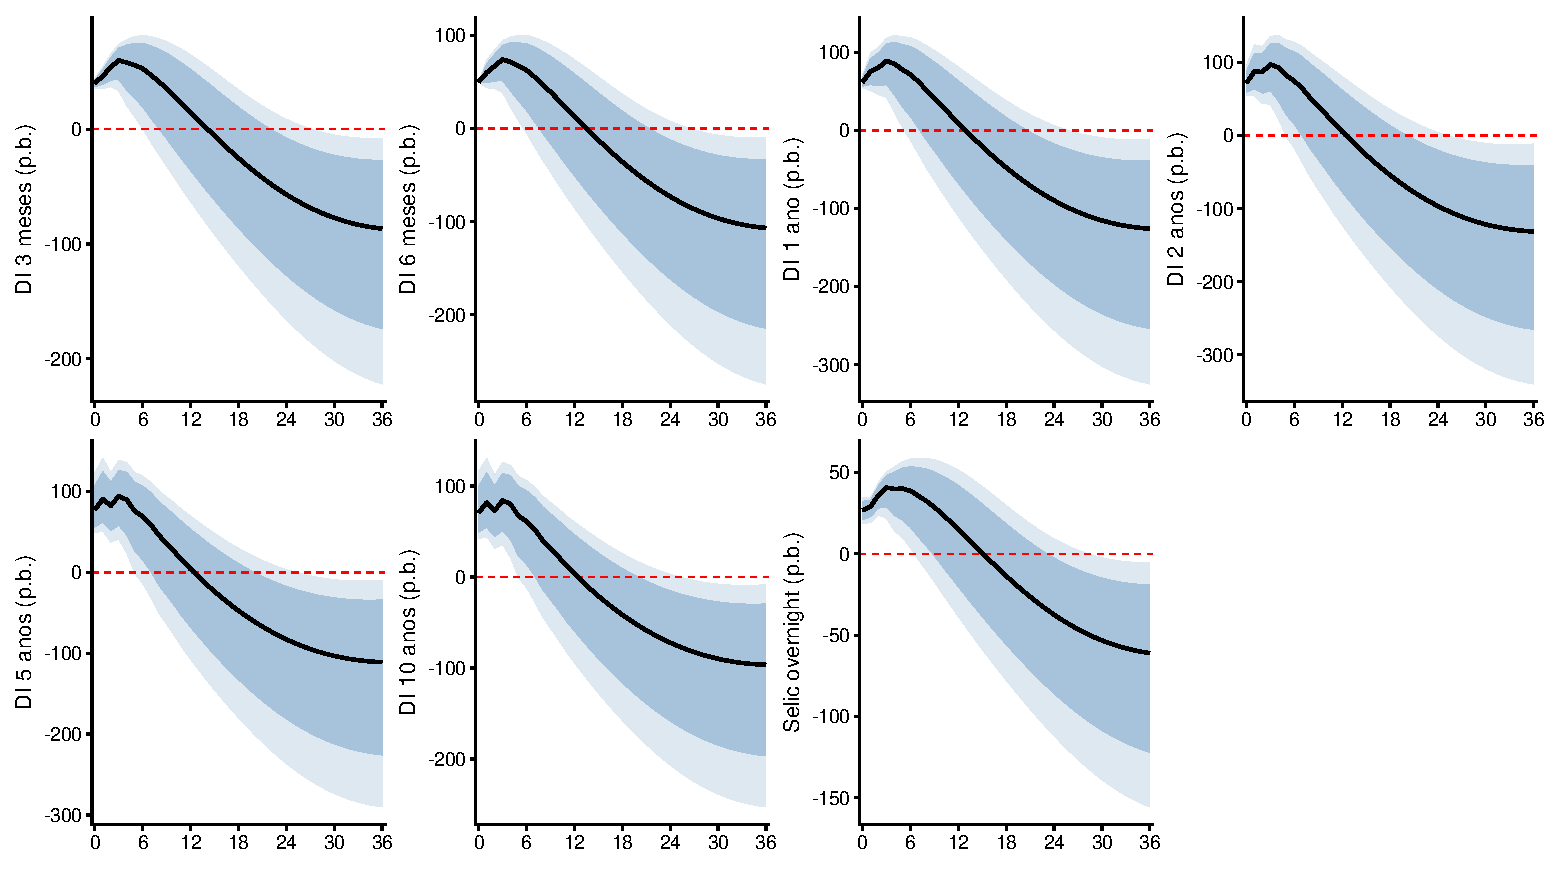
\includegraphics[scale=0.7]{fig_curva.pdf}
\caption{\textbf{Estrutura a termo}\\{Resposta a um choque contracionista normalizado em 50 pontos-base no DI de 6 meses. A linha preta mostra a estimativa pontual em pontos-base, e as áreas escura e clara mostram os conjuntos Anderson--Rubin de 68\% e 90\%. O conjunto do DI de 6 meses se reduz a um ponto no impacto, fixado pela normalização. A Selic é a taxa \textit{overnight} mensal.}}
%\footnotesize{Source: Own elaboration, based on data from Central Bank.}
\label{fig:curva}
\end{center} 
\end{figure}

\subsection{Câmbio e risco soberano}\label{sec:cambio}
O real se deprecia no impacto contra as cinco moedas observadas, o que indica um movimento da moeda brasileira e não apenas do par com o dólar. As respostas são $3{,}23\%$ no BRL/USD, $2{,}37\%$ no BRL/EUR, $3{,}06\%$ no BRL/CNY, $2{,}61\%$ no BRL/INR e $3{,}59\%$ no BRL/ARS.

A depreciação se intensifica no curto prazo e depois reverte. BRL/EUR, BRL/CNY e BRL/INR atingem picos de $3{,}05\%$, $3{,}87\%$ e $3{,}36\%$ no mês seguinte, e BRL/USD e BRL/ARS alcançam $4{,}03\%$ e $4{,}64\%$ no terceiro mês. As cinco respostas mudam de sinal entre o décimo primeiro e o décimo quarto mês e, no trigésimo sexto, indicam apreciação do real entre $1{,}38\%$ no BRL/EUR e $3{,}89\%$ no BRL/ARS, sem retornar ao eixo dentro da janela da figura. %Para o BRL/USD, a banda de 90\% permanece acima de zero até o quarto mês e a de 68\% até o sétimo. Esta última fica abaixo de zero entre o vigésimo segundo e o trigésimo segundo meses, mas a banda de 90\% abrange zero durante toda a apreciação. Ao final dos quatro anos, o ponto do BRL/USD volta a ser levemente positivo e se aproxima do eixo.

O EMBI+ e o CDS de cinco anos acompanham o câmbio, com alta de $25{,}1$ e $30{,}5$ pontos-base no impacto (\autoref{fig:cambio}) e picos de $26{,}8$ e $33{,}5$ no mês seguinte. Os dois cruzam zero no décimo quarto mês, o mesmo do BRL/ARS e um mês depois do BRL/USD, e continuam a cair até o fim do horizonte, com $-17{,}2$ e $-23{,}5$ pontos-base no trigésimo sexto mês.


%  A resposta cambial de impacto equivale a $7{,}48\%$ de depreciação por 100 pontos-base de choque, enquanto \cite{goncalves2025} estimam apreciação entre $3{,}4\%$ e $5{,}6\%$ com dados diários. Como frequência, amostra e estratégia de identificação diferem simultaneamente, essa divergência de sinal não permite atribuir o contraste a um único mecanismo.

\begin{figure}[H]
\begin{center}
    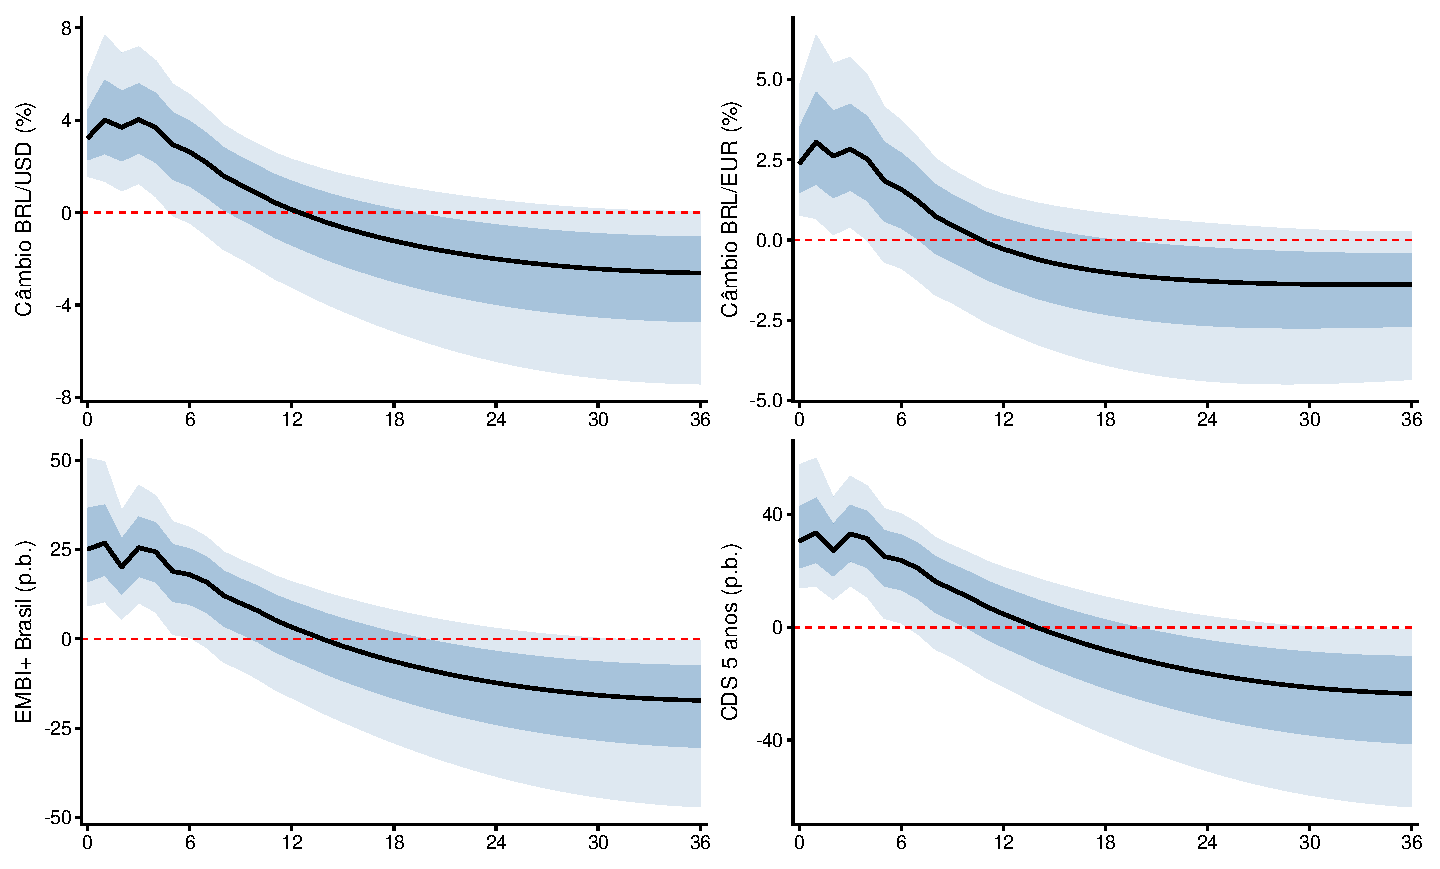
\includegraphics[scale=0.7]{fig_cambio_risco.pdf}
\caption{\textbf{Câmbio e risco soberano}\\{A linha preta mostra a estimativa pontual, e as áreas escura e clara mostram os conjuntos Anderson--Rubin de 68\% e 90\%. As taxas de câmbio em nível são divididas pela respectiva média amostral e expressas em percentual, com valores positivos indicando depreciação do real. EMBI+ e CDS são expressos em pontos-base.}}
%\footnotesize{Source: Own elaboration, based on data from Central Bank.}
\label{fig:cambio}
\end{center} 
\end{figure}

\subsection{Variáveis fiscais}

A DLSP cai $0{,}67$ ponto percentual do PIB no impacto, atinge o vale de $-0{,}79$ no terceiro mês, cruza zero no décimo sexto e chega a $0{,}66$ no trigésimo sexto. A DBGG cai $0{,}17$ ponto percentual do PIB no impacto, atinge o vale de $-0{,}45$ no quinto mês, cruza zero no décimo nono e alcança $0{,}59$ no trigésimo sexto (\autoref{fig:fiscal}).

A NFSP primária cai R\$ $1{,}47$ bilhão no impacto, atinge o vale de R\$ $-3{,}37$ bilhões no mês seguinte, cruza zero no oitavo mês e alcança o pico de R\$ $4{,}63$ bilhões no vigésimo sétimo, com R\$ $4{,}17$ bilhões no trigésimo sexto. O conjunto de 90\% exclui zero no mês seguinte ao choque e do décimo oitavo ao trigésimo segundo mês.

O ajuste cambial cai R\$ $20{,}8$ bilhões no impacto, com conjunto de 68\% entre R\$ $-45{,}4$ e R\$ $-1{,}0$ bilhão, e o conjunto de 90\% contém zero em todos os horizontes.

\begin{figure}[H]
\begin{center}
    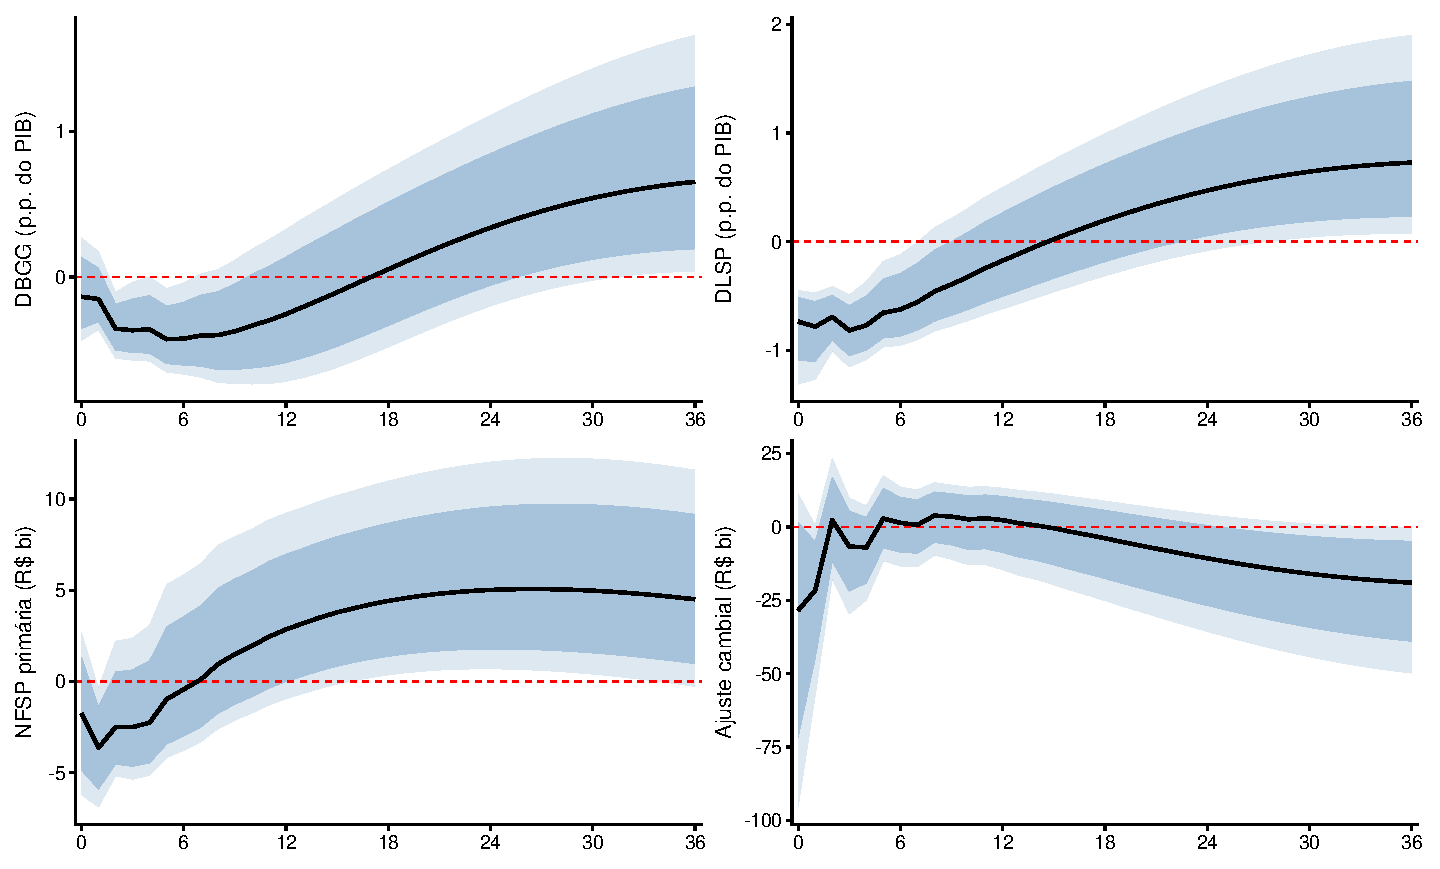
\includegraphics[scale=0.7]{fig_fiscal.pdf}
\caption{\textbf{Variáveis fiscais}\\{A linha preta mostra a estimativa pontual, e as áreas escura e clara mostram os conjuntos Anderson--Rubin de 68\% e 90\%. DBGG e DLSP são expressas em pontos percentuais do PIB, e a NFSP primária e o ajuste cambial, em R\$ bilhões.}}
\label{fig:fiscal}
\end{center}
\end{figure}

\subsection{Expectativas Focus}

No impacto, a expectativa de IPCA para 12 meses sobe $0{,}093$ ponto percentual, atinge $0{,}182$ no terceiro mês, cruza zero no décimo segundo e chega a $-0{,}348$ no trigésimo sexto. A expectativa da Selic para o ano seguinte aumenta $0{,}448$ ponto percentual no impacto, chega a $0{,}644$ no terceiro mês, cruza zero no décimo sexto e atinge $-0{,}703$ no trigésimo sexto. A expectativa de PIB para o ano seguinte cai $0{,}179$ ponto percentual no impacto, atinge o vale de $-0{,}265$ no terceiro mês, cruza zero no décimo sexto e chega a $0{,}274$ no trigésimo sexto (\autoref{fig:expectativas}).

Para o câmbio do ano seguinte, a expectativa sobe R\$ $0{,}074$/US\$ no impacto, alcança R\$ $0{,}107$/US\$ no terceiro mês, cruza zero no décimo segundo e chega a R\$ $-0{,}114$/US\$ no trigésimo sexto.

A expectativa de DLSP cai $0{,}208$ ponto percentual do PIB no impacto, atinge o vale de $-0{,}261$ no quarto mês e cruza zero no décimo sexto. Seu conjunto de 90\% exclui zero apenas no impacto.

O resultado primário esperado cai $0{,}020$ ponto percentual do PIB no impacto, atinge o vale de $-0{,}051$ no segundo mês e cruza zero no décimo quarto. Seu conjunto de 68\% exclui zero do primeiro ao quinto mês, e o de 90\% contém zero em todo o horizonte. O resultado nominal esperado cai $0{,}123$ ponto percentual do PIB no impacto, alcança o vale de $-0{,}194$ no terceiro mês e cruza zero no décimo quinto. Seu conjunto de 90\% exclui zero do impacto ao sexto mês e volta a excluí-lo a partir do trigésimo, com sinal positivo.

\begin{figure}[H]
\begin{center}
    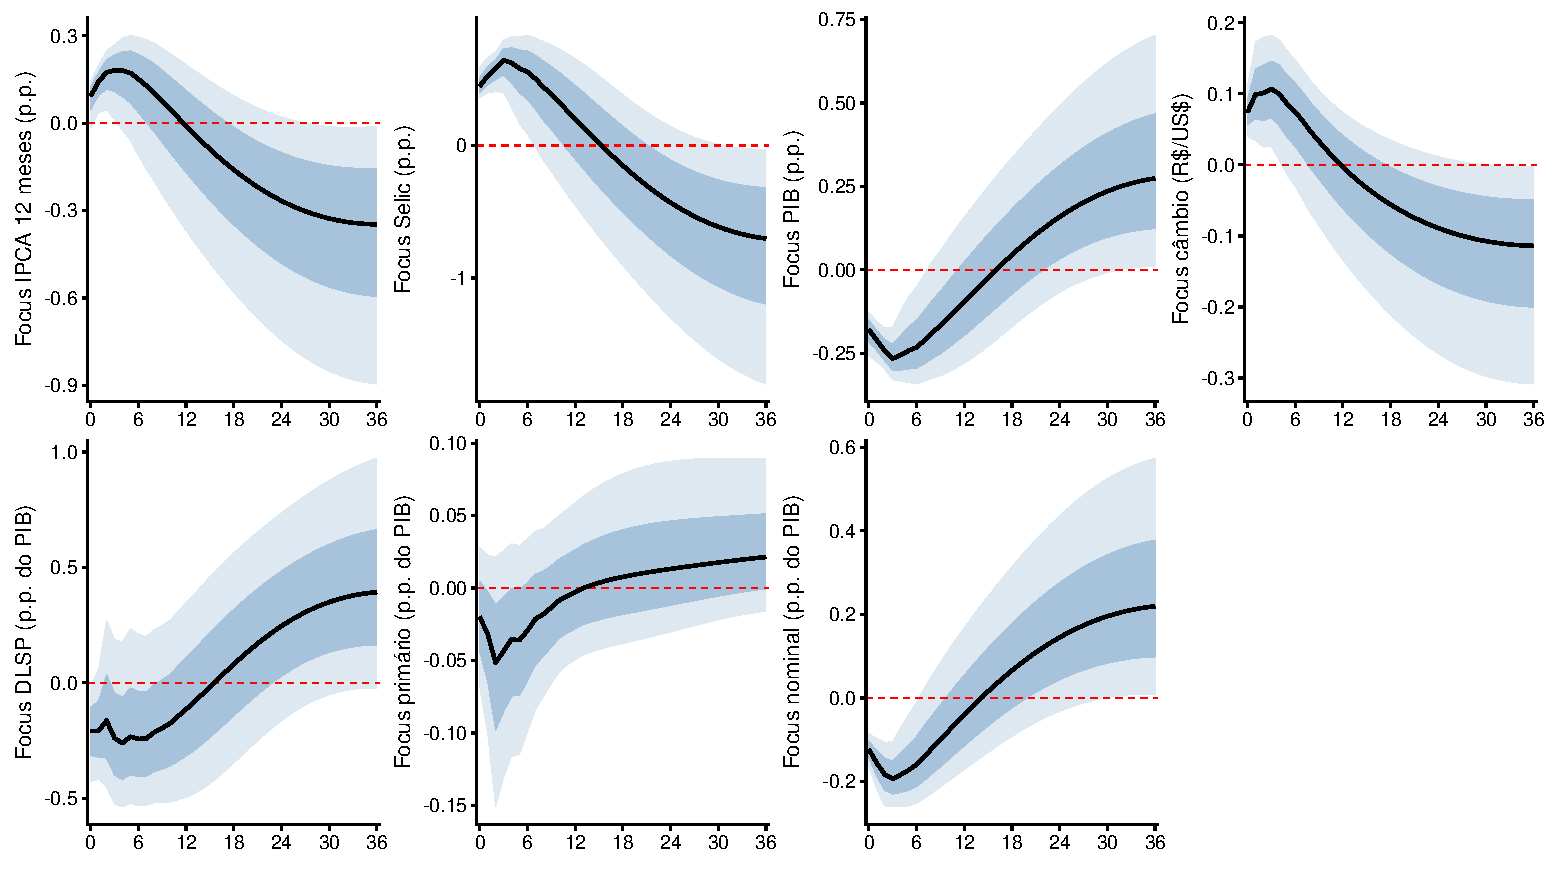
\includegraphics[scale=0.7]{fig_expectativas.pdf}
\caption{\textbf{Expectativas Focus}\\{A linha preta mostra a estimativa pontual, e as áreas escura e clara mostram os conjuntos Anderson--Rubin de 68\% e 90\%. IPCA, Selic e PIB são expressos em pontos percentuais, o câmbio em R\$/US\$, e as três expectativas fiscais em pontos percentuais do PIB. IPCA se refere ao horizonte de 12 meses, enquanto as demais expectativas se referem ao ano seguinte.}}
\label{fig:expectativas}
\end{center}
\end{figure}

\subsection{Atividade e mercado de trabalho}

A atividade recua no impacto em todas as medidas, embora a magnitude varie entre produção, consumo, serviços e utilização de insumos. O IBC-Br cai $0{,}66\%$, a indústria de transformação $2{,}07\%$, os bens duráveis $6{,}01\%$ e os bens de capital $3{,}43\%$. No consumo, as vendas no varejo recuam $1{,}22\%$ e as vendas de serviços $0{,}69\%$, enquanto a utilização da capacidade cai $0{,}23$ ponto percentual e as horas trabalhadas na indústria, $1{,}23\%$ (\autoref{fig:atividade}).

O IBC-Br não muda de sinal em nenhum horizonte. A contração se atenua para $-0{,}44\%$ no mês seguinte, volta a se aprofundar a partir do terceiro e alcança um segundo vale de $-0{,}61\%$ no décimo sexto mês, menor que o impacto em valor absoluto. A recuperação posterior é gradual, e a resposta ainda está em $-0{,}55\%$ depois de dois anos e em $-0{,}33\%$ depois de três. O conjunto de 90\% exclui zero no impacto, no terceiro mês e do sexto ao vigésimo quarto.

Indústria de transformação, bens duráveis, bens de capital, varejo e horas trabalhadas seguem o mesmo desenho, com alívio no primeiro e no segundo mês e um segundo vale entre o décimo e o décimo segundo mês que supera o impacto em valor absoluto. A indústria de transformação chega a $-2{,}15\%$ e os bens de capital a $-4{,}09\%$ no décimo segundo mês, e os bens duráveis, a $-6{,}64\%$ no décimo. O varejo e as horas trabalhadas voltam a $-1{,}26\%$ e $-1{,}30\%$ no décimo segundo mês, pouco abaixo do impacto. Nenhuma dessas respostas cruza zero em três anos, e no trigésimo sexto mês elas vão de $-0{,}24\%$ nas horas trabalhadas a $-0{,}91\%$ nos bens de capital.

As vendas de serviços têm o vale mais tardio do bloco, de $-1{,}00\%$ no vigésimo quarto mês, e ainda estão em $-0{,}83\%$ no trigésimo sexto. A utilização da capacidade atinge $-0{,}32$ ponto percentual no décimo segundo mês. Os conjuntos de 90\% da indústria de transformação, dos bens duráveis e de capital, da utilização da capacidade e das horas trabalhadas excluem zero no impacto e, depois de um ou dois meses de alívio, até pelo menos o vigésimo segundo mês. O do varejo exclui zero sem interrupção do impacto ao vigésimo terceiro mês, e o das vendas de serviços, apenas do décimo sexto ao vigésimo sétimo.

\begin{figure}[H]
\begin{center}
    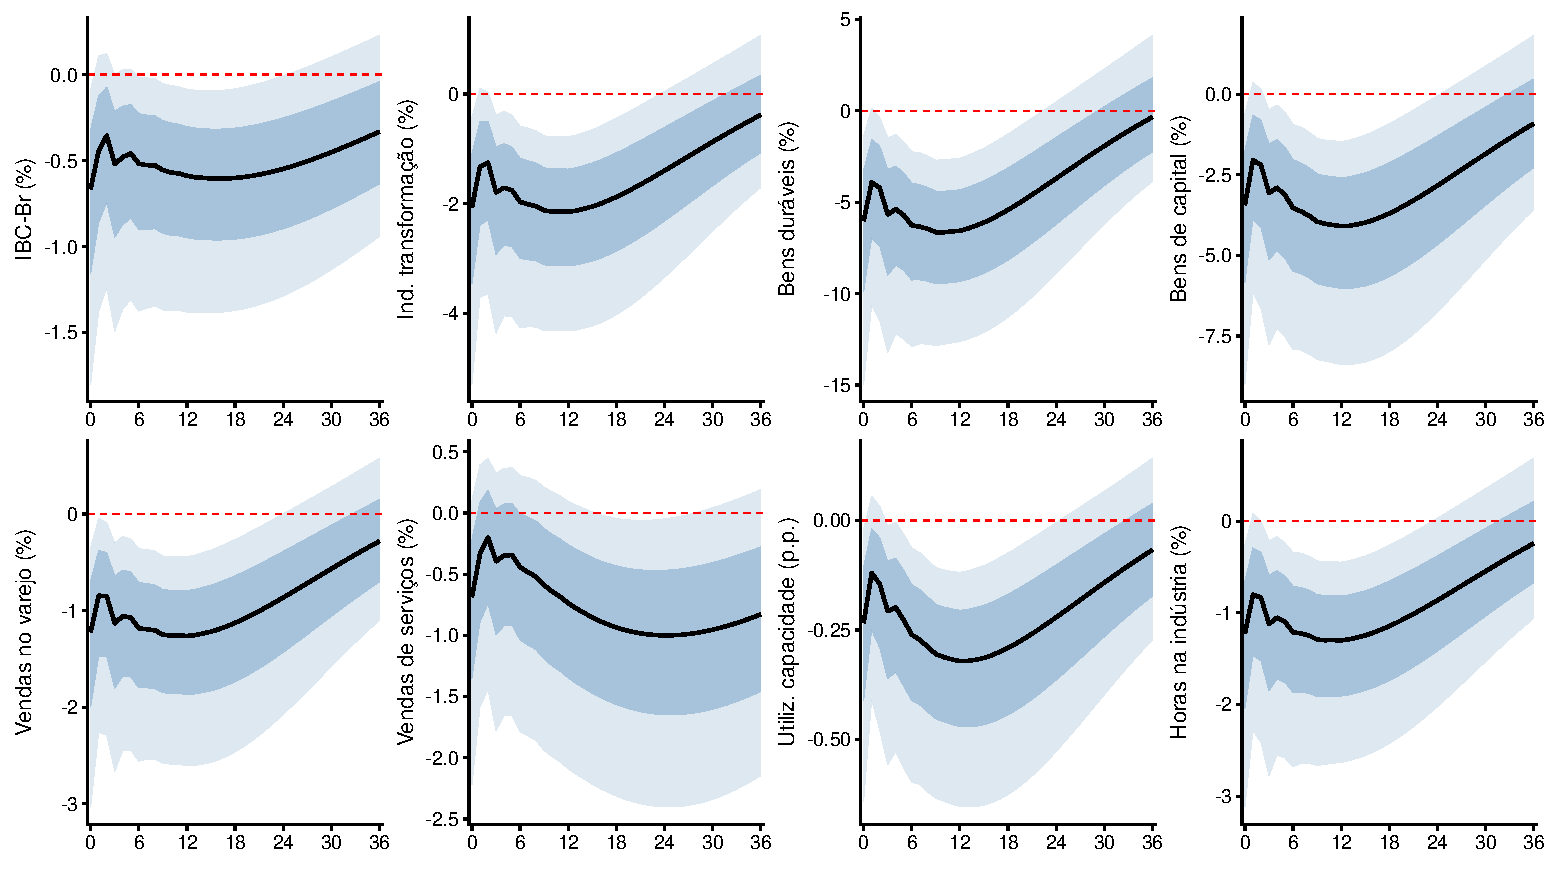
\includegraphics[scale=0.7]{fig_atividade.pdf}
\caption{\textbf{Atividade e horas trabalhadas}\\{A linha preta mostra a estimativa pontual, e as áreas escura e clara mostram os conjuntos Anderson--Rubin de 68\% e 90\%. Índices de atividade, produção, vendas e horas são divididos pela respectiva média amostral e expressos em percentual. A utilização da capacidade instalada é expressa em pontos percentuais.}}
%\footnotesize{Source: Own elaboration, based on data from Central Bank.}
\label{fig:atividade}
\end{center} 
\end{figure}

\subsection{Crédito}

O crédito cresce de forma generalizada no impacto. O saldo total aumenta $0{,}51\%$, e as altas setoriais alcançam $0{,}89\%$ no agropecuário, $1{,}17\%$ no transporte, $0{,}72\%$ na indústria, $0{,}65\%$ no comércio e $0{,}61\%$ na construção. O crédito à pessoa física aumenta $0{,}27\%$, a menor resposta inicial do bloco (\autoref{fig:credito}).

Essa expansão continua até o terceiro mês, quando saldo total, agropecuária, transporte, indústria, comércio e construção chegam a $0{,}70\%$, $1{,}11\%$, $1{,}43\%$, $0{,}91\%$, $0{,}95\%$ e $0{,}94\%$, e a pessoa física chega a $0{,}46\%$ no terceiro e no quarto mês. As respostas permanecem positivas nos dez primeiros meses em todos os segmentos.

O comércio cruza zero no décimo primeiro mês, seguido por saldo total, agropecuária, transporte e indústria no décimo terceiro e por construção e pessoa física no décimo quarto. A contração se aprofunda até perto do fim do horizonte, e no trigésimo sexto mês as respostas vão de $-0{,}75\%$ na pessoa física a $-1{,}40\%$ no transporte, sem que nenhum segmento retorne ao eixo.

\begin{figure}[H]
\begin{center}
    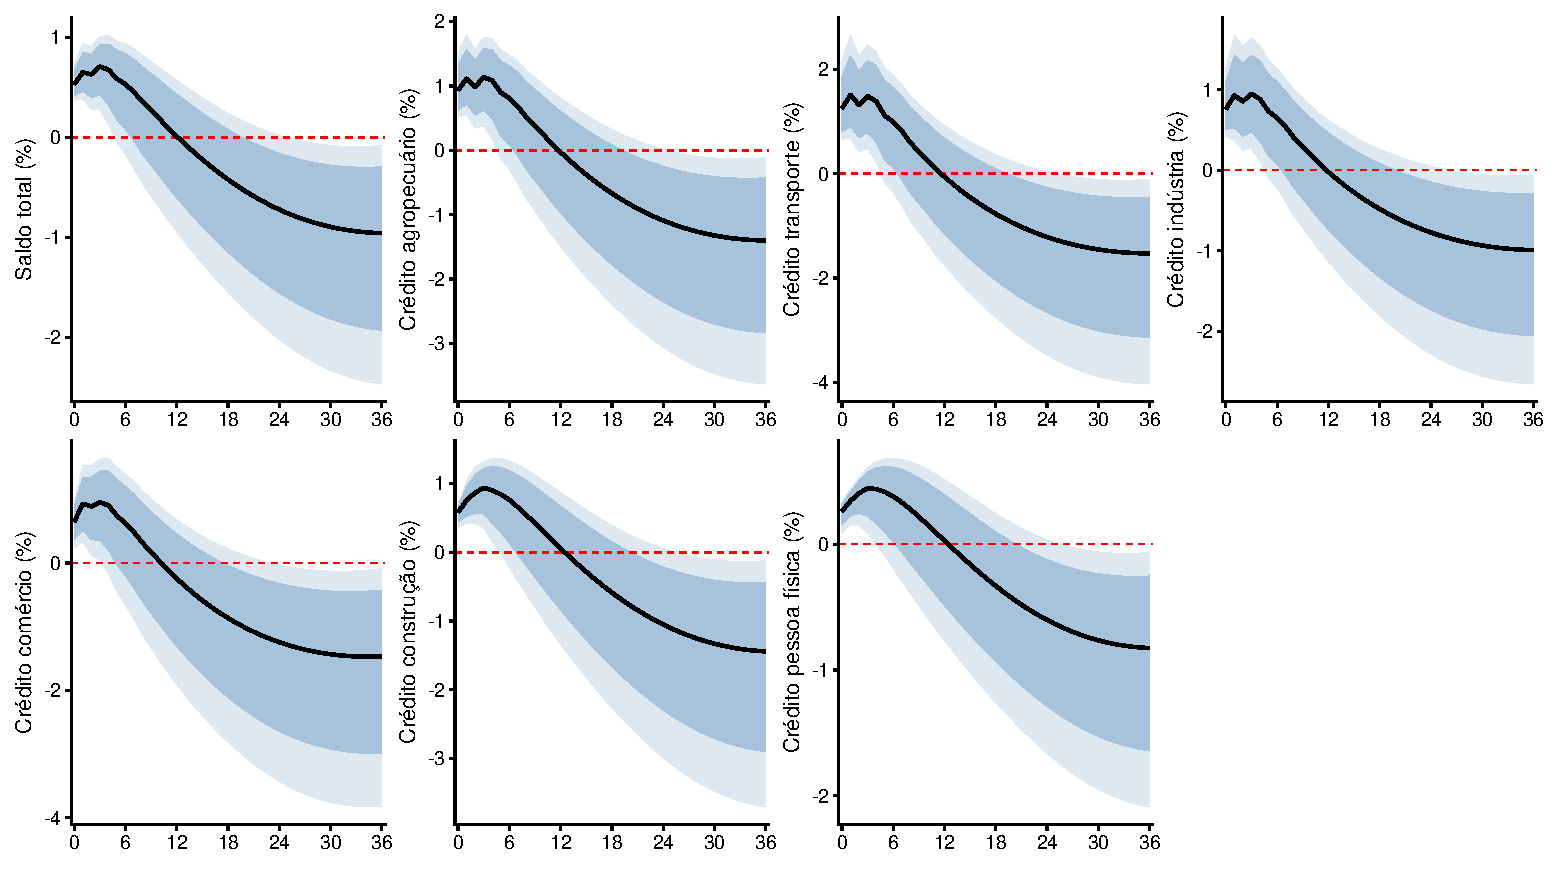
\includegraphics[scale=0.7]{fig_credito.pdf}
\caption{\textbf{Crédito}\\{A linha preta mostra a estimativa pontual, e as áreas escura e clara mostram os conjuntos Anderson--Rubin de 68\% e 90\%. Os saldos entram em log-nível, de modo que as respostas são log-pontos multiplicados por 100 e aproximam variações percentuais.}}
%\footnotesize{Source: Own elaboration, based on data from Central Bank.}
\label{fig:credito}
\end{center} 
\end{figure}

\subsection{Preços}

Os preços ao produtor sobem no impacto, enquanto os preços ao consumidor não exibem a mesma resposta. O IPP aumenta $0{,}342$ ponto percentual e o IGP-M, $0{,}066$, mas o IPCA cheio cai $0{,}045$ ponto percentual, os núcleos EX0 e de médias aparadas ficam próximos de zero, com $0{,}029$ e $0{,}008$, o núcleo EX1 cai $0{,}013$ e o INPC, $0{,}064$ (\autoref{fig:precos}). A diferença entre esses grupos de preços organiza a dinâmica posterior do bloco.

Os preços ao produtor atingem o pico no mês seguinte e mudam de sinal no oitavo. O IPP chega a $0{,}471$ ponto percentual no pico e ao vale de $-0{,}339$ no vigésimo terceiro mês, com $-0{,}280$ no trigésimo sexto. O IGP-M chega a $0{,}167$ no pico e a $-0{,}464$ no trigésimo mês.

O IPCA permanece negativo em todos os horizontes, e a queda se aprofunda a partir do quinto mês, com $-0{,}138$ ponto percentual no décimo segundo e o vale de $-0{,}311$ no trigésimo. No trigésimo sexto mês a resposta ainda está em $-0{,}297$. O núcleo EX1 e o INPC também não mudam de sinal e alcançam vales de $-0{,}165$ e $-0{,}305$ entre o vigésimo sétimo e o trigésimo mês. Os núcleos EX0 e de médias aparadas têm uma alta pequena, de $0{,}060$ no quinto mês e $0{,}028$ no quarto, antes de cruzarem zero no décimo terceiro e no nono. O índice de difusão chega a $0{,}55$ ponto percentual no quarto mês, cruza zero no nono e cai até $-2{,}24$ no trigésimo terceiro.


\begin{figure}[H]
\begin{center}
    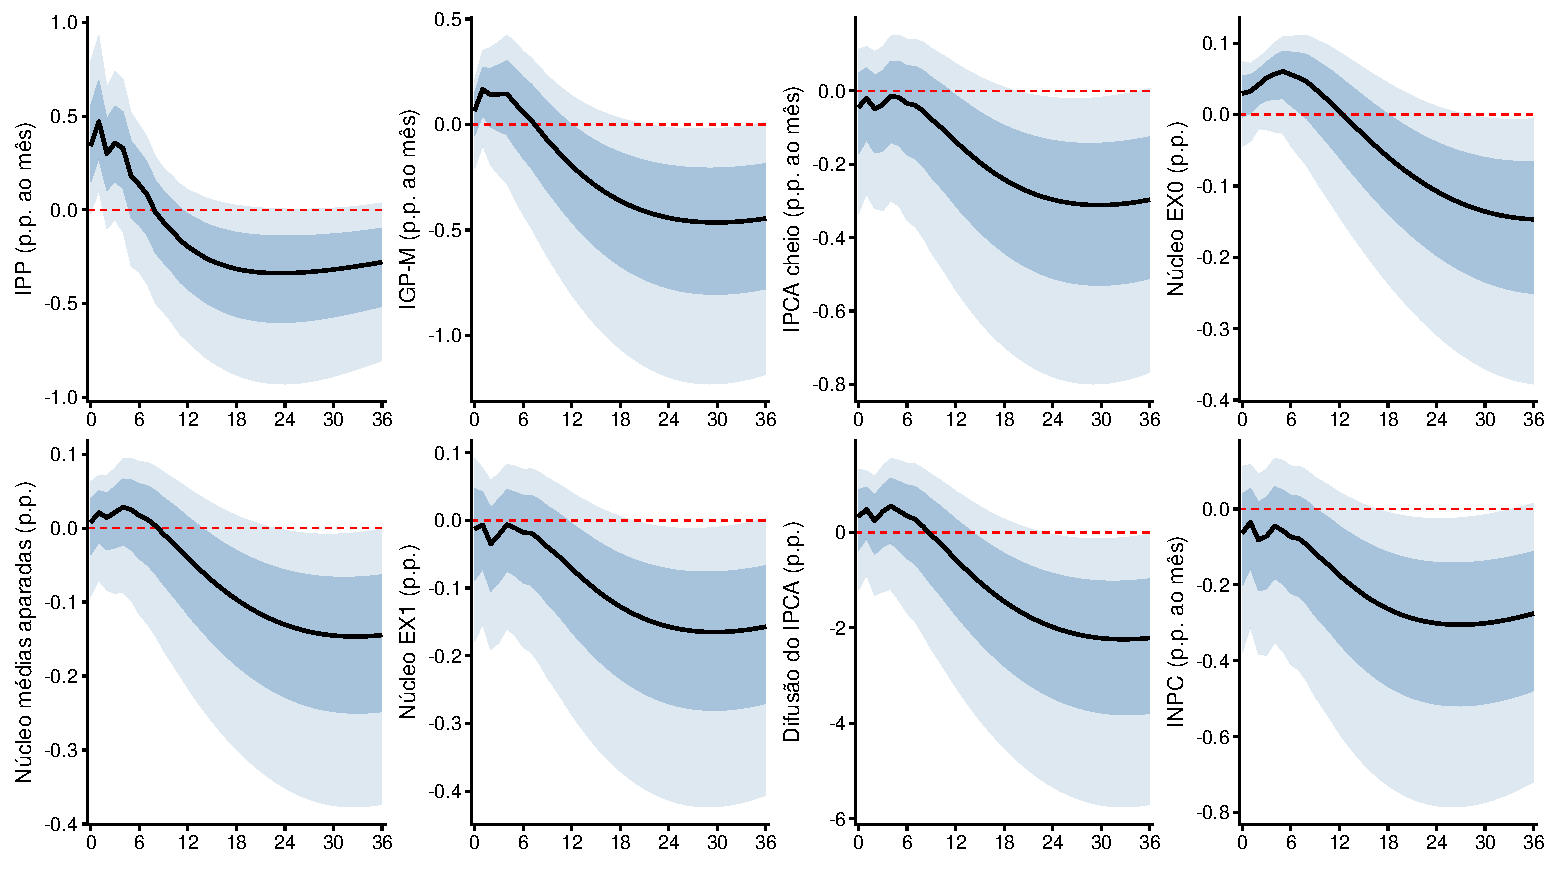
\includegraphics[scale=0.7]{fig_precos.pdf}
\caption{\textbf{Preços}\\{A linha preta mostra a estimativa pontual, e as áreas escura e clara mostram os conjuntos Anderson--Rubin de 68\% e 90\%. As séries de inflação são taxas mensais e as respostas são expressas em pontos percentuais da taxa. O índice de difusão é expresso em pontos percentuais da proporção de itens com aumento de preço.}}
%\footnotesize{Source: Own elaboration, based on data from Central Bank.}
\label{fig:precos}
\end{center} 
\end{figure}

\subsection{Ações}

Seis dos sete índices da B3 têm retorno mensal negativo no impacto. As respostas são $-1{,}50\%$ no Ibovespa, $-2{,}39\%$ no SMLL, $-1{,}83\%$ no IDIV, $-2{,}51\%$ no IMOB, $-2{,}56\%$ no IFNC, $+0{,}09\%$ no IMAT e $-1{,}02\%$ no IFIX (\autoref{fig:acoes}).

Ibovespa, SMLL, IDIV, IMOB e IFNC continuam negativos no mês seguinte e passam ao campo positivo no segundo mês. Depois de uma oscilação entre o terceiro e o quinto mês, em que SMLL e IMOB voltam brevemente ao campo negativo, a fase positiva se firma, com picos de $2{,}18\%$ no Ibovespa, $1{,}85\%$ no IDIV, $1{,}75\%$ no IMOB e $1{,}98\%$ no IFNC no oitavo mês e de $1{,}68\%$ no SMLL no nono. O retorno do IFIX cai a $-1{,}21\%$ no mês seguinte, só se torna positivo no sexto mês e alcança $0{,}48\%$ no décimo segundo.

A fase positiva termina entre o décimo nono e o vigésimo segundo mês, quando os cinco índices voltam ao campo negativo, e o IFIX cruza zero no vigésimo sétimo. No trigésimo sexto mês os sete índices têm retorno negativo, de $-0{,}32\%$ no IFIX a $-3{,}69\%$ no IFNC, com $-2{,}80\%$ no Ibovespa. Como a figura reporta retornos mensais, essa sequência não descreve uma reversão acumulada do nível das ações. O conjunto de 90\% não exclui zero no impacto em nenhum índice. Ele exclui zero na fase positiva do Ibovespa, do quinto ao décimo mês, do SMLL, no oitavo e no nono, e do IDIV, no quinto, no oitavo e no nono, e não exclui zero em nenhum horizonte no IMOB e no IFNC. No IFIX, exclui zero no mês seguinte ao choque, com sinal negativo, e do décimo primeiro ao décimo quarto mês, com sinal positivo.

O IMAT segue trajetória própria, pois seu retorno sobe $0{,}09\%$ no impacto e atinge $2{,}50\%$ no segundo mês, antes de cruzar zero no vigésimo terceiro e chegar a $-1{,}81\%$ no trigésimo sexto. Seu conjunto de 90\% exclui zero no segundo mês e do quarto ao décimo terceiro. Como as empresas do índice recebem parte de sua receita em dólar, a depreciação do real é compatível com esse amortecimento inicial.

\begin{figure}[H]
\begin{center}
    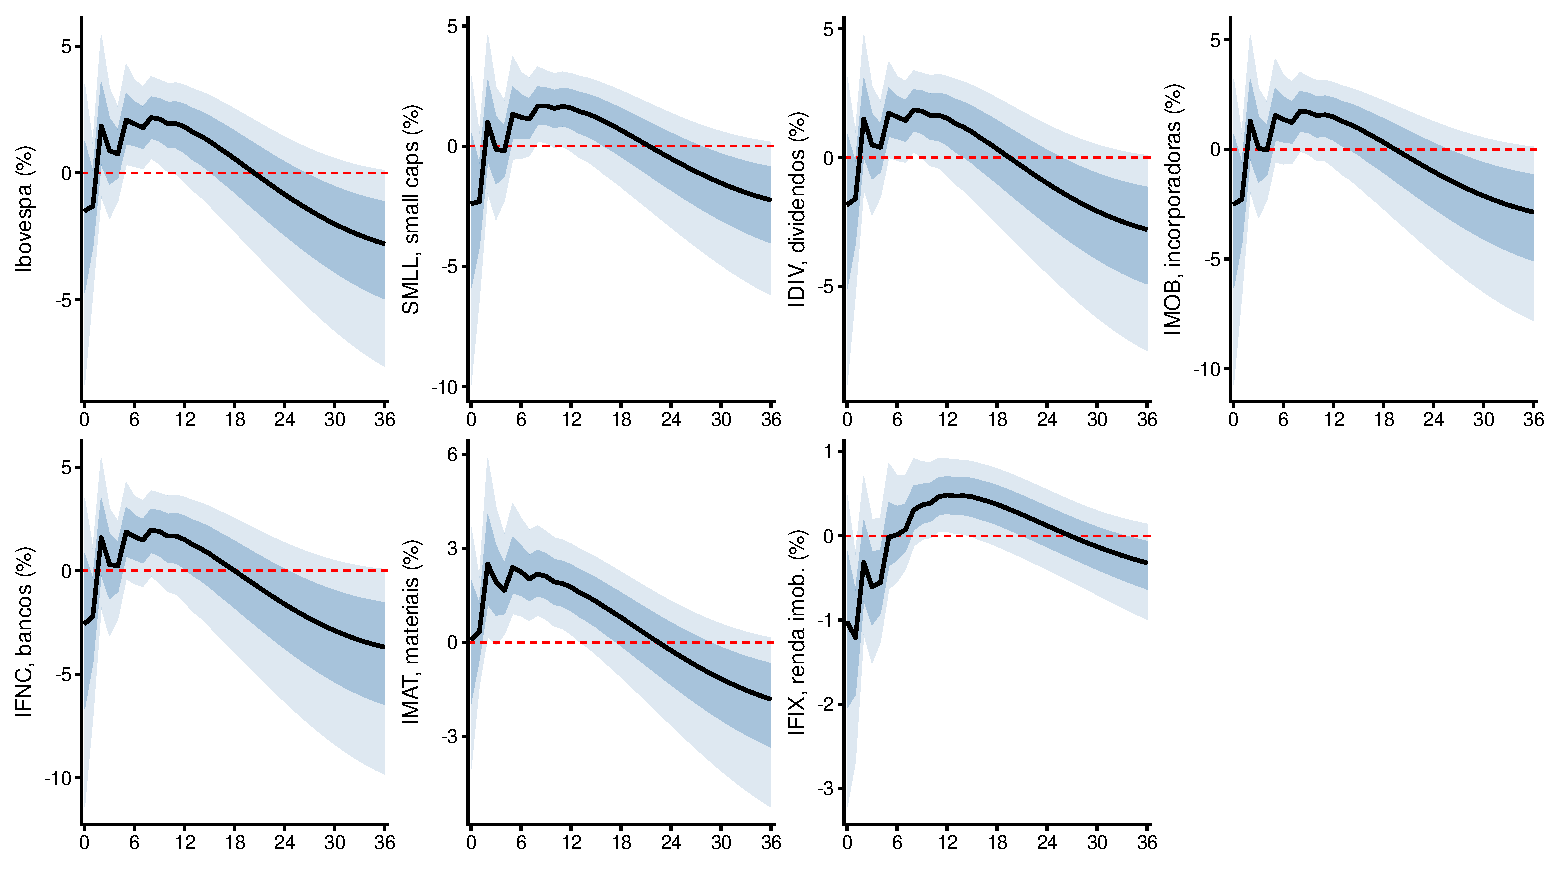
\includegraphics[scale=0.7]{fig_acoes.pdf}
\caption{\textbf{Índices de ações}\\{A linha preta mostra a resposta do retorno mensal em pontos percentuais, sem acumulação ao longo dos horizontes. As áreas escura e clara mostram os conjuntos Anderson--Rubin de 68\% e 90\%.}}
%\footnotesize{Source: Own elaboration, based on data from Central Bank.}
\label{fig:acoes}
\end{center} 
\end{figure}

\section{Robustez}
\label{sec:robustez}
\label{sec:weak_iv}

Os cinco sinais de impacto coincidem entre o DFM e um VAR de cinco observáveis estimado com o mesmo instrumento, e as magnitudes diferem (\autoref{fig:weak_iv_main}). O VAR contém IBC-Br, IPCA, yield de 6 meses, câmbio BRL/USD e CDS soberano de cinco anos em nível, com constante e tendência linear em cada equação, e recebe a mesma normalização de 50 pontos-base. Os conjuntos Anderson--Rubin de \cite{montielolea} são a inferência dos dois lados.

A coincidência entre os modelos não testa a exogeneidade do instrumento. Ambos usam o mesmo $z_t$, e um instrumento contaminado falha nos dois, de modo que o acordo entre eles autoriza apenas dizer que o padrão central sobrevive à inferência robusta a instrumento fraco em uma especificação alternativa de dimensão menor.

Os dois sistemas usam a mesma janela, 2012:03--2025:12 com 162 observações efetivas, e quatro defasagens em cada modelo, como em \cite{alessi}. No VAR essa ordem é escolha de comparabilidade e não do critério de informação, uma vez que na amostra comum de 154 observações o AIC seleciona duas defasagens, com $-11{,}106$ contra $-11{,}006$ em quatro, e o BIC seleciona uma. Com janela e dinâmica comuns, o contraste deixa de misturar amostra e defasagens, embora ainda não isole o conjunto informacional, porque o DFM responde por cinco fatores extraídos de 115 séries e o VAR por cinco observáveis.

No impacto, o IBC-Br cai $0{,}66\%$ da média no DFM e $0{,}73\%$ no VAR, e o IPCA recua $0{,}045$ ponto percentual no DFM contra $0{,}0004$ no VAR. O yield de 6 meses sobe 50 pontos-base nos dois modelos por normalização, o câmbio BRL/USD aumenta $3{,}23\%$ da média no DFM e $2{,}02\%$ no VAR, e o CDS sobe $30{,}5$ e $15{,}7$ pontos-base.

Ao longo do primeiro ano o IPCA separa os dois modelos, subindo a $0{,}109$ ponto percentual no segundo mês no VAR e permanecendo negativo em todo o horizonte no DFM, onde alcança $-0{,}138$ no décimo segundo mês. O IBC-Br não volta a ser positivo em nenhum dos dois, mas se aproxima do eixo mais rápido no VAR, que chega a $-0{,}04\%$ da média no quarto mês contra $-0{,}48\%$ no DFM. O yield de 6 meses é mais persistente no VAR, que atinge $106{,}3$ pontos-base no nono mês, contra o pico de $74{,}0$ no terceiro mês no DFM. Para o câmbio e o CDS, os pontos do DFM são maiores nos primeiros meses, com picos de $4{,}03\%$ e $33{,}5$ pontos-base contra $2{,}85\%$ e $22{,}1$ no VAR. Ao final de três anos as cinco respostas são negativas nos dois modelos.

Os conjuntos de 90\% não formam blocos contíguos, de modo que a persistência se lê horizonte por horizonte. No DFM, o conjunto do IBC-Br exclui zero no impacto, no terceiro mês e entre o sexto e o vigésimo quarto. Os do yield de 6 meses e do CDS excluem zero do impacto ao sexto mês e voltam a excluir a partir do trigésimo e do trigésimo primeiro, já com pontos negativos, enquanto o do câmbio exclui zero do impacto ao quarto mês. O do IPCA não exclui zero no impacto, mas exclui entre o vigésimo e o trigésimo quarto mês, também no ramo negativo. No VAR, o conjunto do IBC-Br exclui zero apenas no impacto, o do yield até o oitavo mês, o do câmbio até o sétimo e o do CDS até o décimo quarto, com uma única lacuna no segundo. O IPCA é o contraste mais nítido, porque no VAR seu conjunto de 90\% exclui zero no segundo e no quarto mês com sinal positivo, o padrão de \textit{price puzzle} que o DFM não apresenta.

\begin{figure}[H]
\begin{center}
    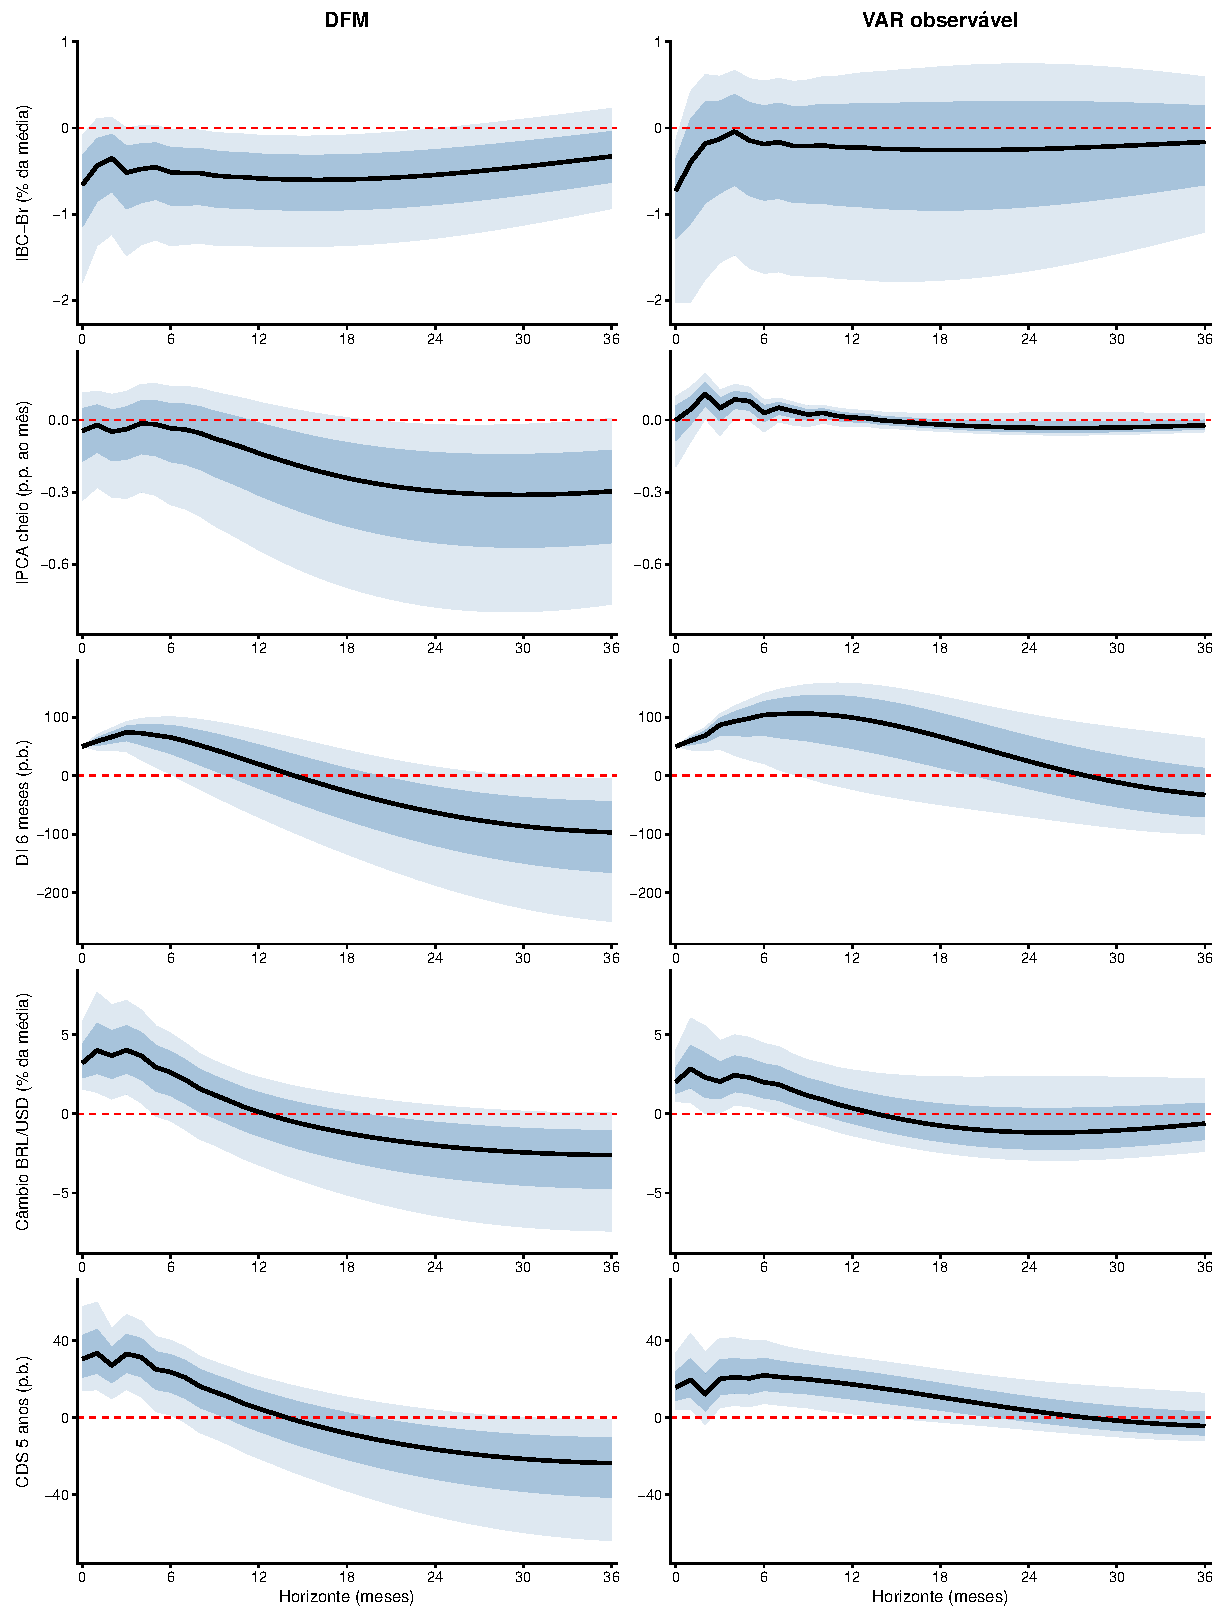
\includegraphics[scale=0.62]{fig_weak_iv_main.pdf}
\caption{\textbf{DFM e benchmark VAR observável}\\{Respostas a um choque de 50 pontos-base no DI de seis meses. As faixas de 68\% e 90\% são conjuntos Anderson--Rubin com NW(0) nos dois modelos. Cada linha usa a mesma escala nos dois modelos, e a linha tracejada marca zero.}}
\label{fig:weak_iv_main}
\end{center}
\end{figure}


%---------------
\section{Concluding remarks}
%%---------------
Este artigo documenta um fato estilizado que contraria o mecanismo convencional da paridade descoberta de juros: em uma economia emergente com histórico de fragilidade fiscal, um aperto monetário pode elevar o prêmio de risco soberano a ponto de depreciar, em vez de apreciar, a moeda doméstica. Usando um modelo de fatores dinâmicos estruturais identificado por instrumento externo sobre um painel de mais de 100 séries macroeconômicas e financeiras brasileiras, mostramos que um choque contracionista de 50 pontos-base deprecia o real em $3,\!23\%$ no impacto, ao mesmo tempo em que o EMBI+ e o CDS soberano de cinco anos se abrem, uma resposta conjunta incompatível com o canal tradicional do diferencial de juros, mas consistente com um regime em que o aumento da taxa de juros piora a percepção sobre a sustentabilidade da dívida.

A curva de juros reforça essa interpretação. O repasse do choque cresce com a maturidade até cinco anos, superando a amplificação documentada para economias desenvolvidas. No médio prazo, as taxas de juros e as medidas de risco soberano exibem uma dinâmica de reversão altamente sincronizada, ao passo que o câmbio perde significância estatística bem antes dessa reversão, sugerindo que o aumento do prêmio de risco é mais persistente do que seu repasse à taxa de câmbio.

%A curva de juros reforça essa leitura. O repasse do choque cresce com a maturidade até cinco anos, superando a amplificação que desenhos comparáveis encontram em economias desenvolvidas, e reverte no médio prazo em estreita sincronia com o câmbio e o prêmio de risco soberano, os cinco vértices, o EMBI+ e o CDS revertem de sinal em janelas próximas, entre o décimo e o vigésimo quarto mês. O câmbio, no entanto, não acompanha essa reversão: sua resposta perde significância estatística já a partir do quinto mês, sugerindo que o efeito sobre o risco soberano é mais persistente do que seu repasse ao câmbio.

Os demais resultados sugerem que esse canal de prêmio de risco opera em paralelo aos canais tradicionais de transmissão da política monetária. A atividade econômica desacelera, o mercado de trabalho responde com defasagem, o crédito inicialmente se expande antes de contrair de forma mais disseminada, e a inflação ao produtor apresenta evidências de repasse cambial no curto prazo, o mercado acionário é a exceção, sem resposta de impacto estatisticamente significativa em nenhum dos sete índices analisados. Em conjunto, esses resultados indicam que o aumento do prêmio de risco soberano não substitui os canais convencionais de transmissão, mas passa a coexistir com eles em contextos de fragilidade fiscal como o brasileiro.

Nossos resultados contrastam com evidências recentes para o Brasil obtidas por identificação via heterocedasticidade em frequência diária, que rejeitam a hipótese de dominância fiscal \citep[]{goncalves2025}. A tentativa de transportar essa identificação para o painel mensal mostra que a condição de posto de que a heterocedasticidade depende vale nas três séries em frequência diária e falha nas mesmas três séries no painel mensal, onde os dois maiores autovalores praticamente coincidem, que é a proporcionalidade apontada por \cite{rigobon2003}. A divergência entre os resultados é compatível com a representação fatorial e com a propagação captada pelo modelo, sem autorizar a heterocedasticidade como estratégia alternativa para este artigo.

Do ponto de vista de política econômica, nossos resultados indicam que, em economias emergentes sujeitas a fragilidades fiscais, a eficácia do canal cambial da política monetária não deve ser assumida automaticamente a partir do mecanismo convencional da paridade descoberta da taxa de juros. Nesses contextos, a credibilidade fiscal, e não apenas a magnitude do choque monetário, passa a condicionar a direção da resposta cambial. Mais amplamente, nossos resultados sugerem que a transmissão da política monetária deve ser compreendida como o resultado da interação entre política monetária e percepção de risco soberano, e não apenas como consequência do diferencial de juros. Essa perspectiva amplia a interpretação tradicional do canal cambial e, no caso brasileiro, oferece uma explicação alternativa para episódios em que aumentos da taxa básica de juros são acompanhados por depreciação cambial, um padrão que pode ser relevante para outras economias emergentes sujeitas a preocupações semelhantes de sustentabilidade fiscal.

%\section*{Funding}
%Jo\~ao F. Caldeira gratefully acknowledges support provided by CNPq under grant 309448/2022-0.

%%---------------
%% Bibliografia
%%---------------
%\section*{References}
\bibliographystyle{authordate3} % bibliography style
\bibliography{references} % References file

\section*{Anexo A. Lista de variáveis}\label{anexo-A}

\begin{ThreePartTable}
\begin{TableNotes}
\footnotesize
\item[*] Código de transformação com que a série entra na extração de fatores e é recuperada em unidades econômicas na função de impulso-resposta. 1 = nível. 2 = retorno mensal, com a função de impulso-resposta acumulada para recuperar a resposta de nível de preço. 4 = log-nível. Os índices de mercado da B3 entram como retorno mensal. Os volumes nominais (base monetária, agregados, crédito, PIB e recolhimentos compulsórios) entram em logaritmo. As séries com sazonalidade detectada são ajustadas por X-13ARIMA-SEATS \cite{sax2018seasonal}. Todas as séries são padronizadas pelo desvio padrão da primeira diferença \cite{barigozzi2016non} antes da extração de fatores. As séries em nível não são diferenciadas, a não-estacionariedade é acomodada pela padronização.
\end{TableNotes}

\footnotesize
\setlength{\tabcolsep}{4pt}
\begin{longtable}{@{}p{5.2cm} l l c@{}}
\caption{Lista de Variáveis Utilizadas}\label{tab:lista_variaveis} \\
\toprule
\textbf{Variável} & \textbf{Fonte} & \textbf{Grupo} & \textbf{Código} \\
\midrule
\endfirsthead

\toprule
\textbf{Variável} & \textbf{Fonte} & \textbf{Grupo} & \textbf{Código} \\
\midrule
\endhead



\bottomrule
\insertTableNotes
\endlastfoot

Câmbio USD/BRL & Yahoo Finance & Câmbio & 1 \\
Câmbio EUR/BRL & Yahoo Finance & Câmbio & 1 \\
Câmbio CNY/BRL & Yahoo Finance & Câmbio & 1 \\
Câmbio ARS/BRL & Yahoo Finance & Câmbio & 1 \\
Câmbio INR/BRL & Yahoo Finance & Câmbio & 1 \\
Selic (meta acumulada) & BCB (4189) & Juros e curva & 1 \\
CDI acumulado & BCB (4392) & Juros e curva & 1 \\
DI 3 meses & Svensson/B3 & Juros e curva & 1 \\
DI 6 meses & Svensson/B3 & Juros e curva & 1 \\
DI 1 ano & Svensson/B3 & Juros e curva & 1 \\
DI 2 anos & Svensson/B3 & Juros e curva & 1 \\
DI 5 anos & Svensson/B3 & Juros e curva & 1 \\
DI 10 anos & Svensson/B3 & Juros e curva & 1 \\
Base monetária & BCB (1788) & Agregados monetários & 4 \\
Meios de pagamento & BCB (27789) & Agregados monetários & 4 \\
Depósitos à vista & BCB (27790) & Agregados monetários & 4 \\
Depósitos de poupança & BCB (1835) & Agregados monetários & 4 \\
M1 & BCB (27791) & Agregados monetários & 4 \\
M2 & BCB (27810) & Agregados monetários & 4 \\
M3 & BCB (27813) & Agregados monetários & 4 \\
Crédito agropecuário & BCB (22027) & Crédito & 4 \\
Crédito indústria & BCB (22043) & Crédito & 4 \\
Crédito construção & BCB (22030) & Crédito & 4 \\
Crédito comércio & BCB (22036) & Crédito & 4 \\
Crédito transporte & BCB (22037) & Crédito & 4 \\
Crédito pessoa física & BCB (22050) & Crédito & 4 \\
Spread ICC pessoa jurídica & BCB (27444) & Crédito & 1 \\
Spread ICC pessoa física & BCB (27445) & Crédito & 1 \\
Saldo de crédito total & BCB (20542) & Crédito & 4 \\
Recolhimentos compulsórios & BCB (17633) & Crédito & 4 \\
Consumo de gasolina & BCB (1393) & Atividade econômica & 1 \\
Consumo de GLP & BCB (1394) & Atividade econômica & 1 \\
Consumo de óleo combustível & BCB (1395) & Atividade econômica & 1 \\
Consumo de óleo diesel & BCB (1396) & Atividade econômica & 1 \\
Consumo de demais derivados & BCB (1397) & Atividade econômica & 1 \\
Consumo de álcool & BCB (1401) & Atividade econômica & 1 \\
Utilização da capacidade instalada (CNI) & BCB (28554) & Atividade econômica & 1 \\
Vendas no varejo & BCB (1455) & Atividade econômica & 1 \\
Vendas de serviços & BCB (23982) & Atividade econômica & 1 \\
Produção de automóveis & BCB (7384) & Atividade econômica & 1 \\
Produção de veículos leves & BCB (7385) & Atividade econômica & 1 \\
Produção de caminhões & BCB (7386) & Atividade econômica & 1 \\
Produção de ônibus & BCB (7387) & Atividade econômica & 1 \\
Produção de bens de consumo & BCB (21865) & Atividade econômica & 1 \\
Produção de bens duráveis & BCB (21866) & Atividade econômica & 1 \\
Produção de bens não duráveis & BCB (21867) & Atividade econômica & 1 \\
Produção de bens de capital & BCB (21863) & Atividade econômica & 1 \\
Produção da indústria de transformação & BCB (21862) & Atividade econômica & 1 \\
Produção da indústria extrativa & BCB (21861) & Atividade econômica & 1 \\
Utilização da capacidade instalada (FGV) & BCB (24352) & Atividade econômica & 1 \\
Consumo de energia comercial & BCB (1402) & Atividade econômica & 1 \\
Consumo de energia residencial & BCB (1403) & Atividade econômica & 1 \\
Consumo de energia industrial & BCB (1404) & Atividade econômica & 1 \\
Consumo de energia outros & BCB (1405) & Atividade econômica & 1 \\
PIB acumulado no ano & BCB (4381) & Atividade econômica & 4 \\
IBC-Br & BCB (24364) & Atividade econômica & 1 \\
Índice de confiança do consumidor & BCB (4393) & Atividade econômica & 1 \\
Índice de confiança de serviços & BCB (17660) & Atividade econômica & 1 \\
Emprego formal Sudeste & BCB (13901) & Mercado de trabalho & 1 \\
Emprego formal Sul & BCB (13564) & Mercado de trabalho & 1 \\
Emprego formal Nordeste & BCB (13941) & Mercado de trabalho & 1 \\
Emprego formal Norte & BCB (28152) & Mercado de trabalho & 1 \\
Emprego formal Centro-Oeste & BCB (21991) & Mercado de trabalho & 1 \\
Salário mínimo & BCB (1619) & Mercado de trabalho & 1 \\
População na força de trabalho & BCB (24378) & Mercado de trabalho & 1 \\
População ocupada & BCB (28543) & Mercado de trabalho & 1 \\
Taxa de desemprego & BCB (24369) & Mercado de trabalho & 1 \\
Horas trabalhadas na indústria & BCB (28556) & Mercado de trabalho & 1 \\
Tempo de procura: até 1 mês & IBGE/SIDRA (1616) & Mercado de trabalho & 1 \\
Tempo de procura: 1 mês a 1 ano & IBGE/SIDRA (1616) & Mercado de trabalho & 1 \\
Tempo de procura: 1 a 2 anos & IBGE/SIDRA (1616) & Mercado de trabalho & 1 \\
Tempo de procura: 2 anos ou mais & IBGE/SIDRA (1616) & Mercado de trabalho & 1 \\
IPCA & BCB (433) & Inflação & 1 \\
IPCA índice de difusão & BCB (21379) & Inflação & 1 \\
IPCA núcleo EX0 & BCB (29677) & Inflação & 1 \\
IPCA núcleo EX1 & BCB (29678) & Inflação & 1 \\
IPCA núcleo médias aparadas & BCB (16122) & Inflação & 1 \\
IGP-M & BCB (189) & Inflação & 1 \\
IPC & BCB (191) & Inflação & 1 \\
IPC núcleo & BCB (4467) & Inflação & 1 \\
INCC & BCB (192) & Inflação & 1 \\
INPC & BCB (188) & Inflação & 1 \\
IPP & IPEA (IPP12\_IPPCG12) & Inflação & 1 \\
Índice de commodities agropecuária & BCB (27575) & Commodities & 1 \\
Índice de commodities metal & BCB (27576) & Commodities & 1 \\
Índice de commodities energia & BCB (27577) & Commodities & 1 \\
Ibovespa (retorno mensal) & B3 & Índices de mercado & 2 \\
IDIV (retorno mensal) & B3 & Índices de mercado & 2 \\
IFIX (retorno mensal) & B3 & Índices de mercado & 2 \\
IFNC (retorno mensal) & B3 & Índices de mercado & 2 \\
IMAT (retorno mensal) & B3 & Índices de mercado & 2 \\
IMOB (retorno mensal) & B3 & Índices de mercado & 2 \\
MLCX (retorno mensal) & B3 & Índices de mercado & 2 \\
SMLL (retorno mensal) & B3 & Índices de mercado & 2 \\
EMBI+ Brasil & JP Morgan & Risco e incerteza & 1 \\
CDS soberano 5 anos & Investing.com & Risco e incerteza & 1 \\
MSCI mercados emergentes & Investing.com & Risco e incerteza & 1 \\
VIX & CBOE & Risco e incerteza & 1 \\
EPU Brasil & policyuncertainty.com & Risco e incerteza & 1 \\
EPU Canadá & policyuncertainty.com & Risco e incerteza & 1 \\
EPU Chile & policyuncertainty.com & Risco e incerteza & 1 \\
EPU China & policyuncertainty.com & Risco e incerteza & 1 \\
EPU Alemanha & policyuncertainty.com & Risco e incerteza & 1 \\
EPU Índia & policyuncertainty.com & Risco e incerteza & 1 \\
EPU Rússia & policyuncertainty.com & Risco e incerteza & 1 \\
EPU Estados Unidos & policyuncertainty.com & Risco e incerteza & 1 \\

\end{longtable}
\end{ThreePartTable}

\section*{Anexo B. Identificação por heterocedasticidade}\label{anexo-B}

\begin{table}[H]
\begin{center}
\footnotesize
\setlength{\tabcolsep}{5pt}
\begin{threeparttable}
\begin{tabular*}{0.75\textwidth}{@{\extracolsep{\fill}}l l c c c c@{}}
\toprule
\textbf{Sistema} & \textbf{Vértice} & \textbf{$n_C/n_{NC}$} & \textbf{DI} & \textbf{BRL/USD} & \textbf{CDS} \\
\midrule
\multicolumn{6}{@{}l}{\textit{Variação de quarta para quinta-feira}} \\
\quad Diária & 3 meses  & 102/553 & 5{,}54 & 1{,}04 & 0{,}80 \\
\quad Diária & 6 meses  & 102/553 & 2{,}84 & 1{,}04 & 0{,}77 \\
\quad Diária & 12 meses & 102/553 & 2{,}66 & 1{,}04 & 0{,}78 \\
\addlinespace
\multicolumn{6}{@{}l}{\textit{Resíduos do VAR mensal em nível}} \\
\quad Mensal & 3 meses  & 108/54 & 2{,}26 & 1{,}85 & 2{,}42 \\
\quad Mensal & 6 meses  & 108/54 & 2{,}98 & 1{,}86 & 2{,}59 \\
\quad Mensal & 12 meses & 108/54 & 2{,}52 & 1{,}74 & 2{,}59 \\
\bottomrule
\end{tabular*}
\begin{tablenotes}[flushleft]
\footnotesize
\item \textit{Notas:} Razão entre a variância da série nos períodos com reunião do Copom ($C$) e sem reunião ($NC$) \citep{rigobonsack2004}. A coluna DI traz o vértice da linha. No diário, $C$ são semanas com reunião e a série é a variação de quarta para quinta-feira. No mensal, $C$ são meses com reunião e a série é o resíduo de um VAR em nível com constante, tendência e quatro defasagens. As séries são as de \cite{goncalves2025}, sem a expectativa de inflação de mercado, que o painel não contém. Janela 2012:03--2025:12.
\end{tablenotes}
\end{threeparttable}
\caption{\textbf{Razão de variância entre regimes}}
\label{tab:het_variance}
\end{center}
\end{table}

\begin{table}[H]
\begin{center}
\footnotesize
\setlength{\tabcolsep}{4pt}
\begin{threeparttable}
\begin{tabular}{@{}l l c c c c c c c c@{}}
\toprule
 & & & & & & \multicolumn{2}{c}{\textbf{Corrigido}} & \multicolumn{2}{c}{\textbf{Sem correção}} \\
\cmidrule(lr){7-8} \cmidrule(lr){9-10}
\textbf{Sistema} & \textbf{Vértice} & \textbf{$n_C/n_{NC}$} & \textbf{$a$} & \textbf{$\hat{\lambda}_1$} & \textbf{$\hat{\lambda}_2$} & \textbf{$Q_r$} & \textbf{$p$} & \textbf{$Q_r$} & \textbf{$p$} \\
\midrule
\multicolumn{10}{@{}l}{\textit{Variação de quarta para quinta-feira}} \\
\quad Diária & 3 meses & 102/553 & 5{,}54 & 7{,}55 & 1{,}36 & 11{,}43 & 0{,}003 & 55{,}77 & $<0{,}001$ \\
 & & & & (1{,}15) & (0{,}21) & & & & \\
\quad Diária & 6 meses & 102/553 & 2{,}84 & 4{,}06 & 1{,}36 & 4{,}95 & 0{,}084 & 24{,}29 & $<0{,}001$ \\
 & & & & (0{,}62) & (0{,}21) & & & & \\
\quad Diária & 12 meses & 102/553 & 2{,}66 & 3{,}63 & 1{,}40 & 3{,}83 & 0{,}147 & 18{,}51 & $<0{,}001$ \\
 & & & & (0{,}55) & (0{,}21) & & & & \\
\addlinespace
\multicolumn{10}{@{}l}{\textit{VAR mensal em nível}} \\
\quad Mensal & 3 meses & 108/54 & 2{,}26 & 2{,}51 & 2{,}36 & 0{,}02 & 0{,}988 & 0{,}03 & 0{,}983 \\
 & & & & (0{,}59) & (0{,}56) & & & & \\
\quad Mensal & 6 meses & 108/54 & 2{,}98 & 3{,}07 & 2{,}59 & 0{,}17 & 0{,}917 & 0{,}27 & 0{,}876 \\
 & & & & (0{,}73) & (0{,}61) & & & & \\
\quad Mensal & 12 meses & 108/54 & 2{,}52 & 2{,}85 & 2{,}44 & 0{,}14 & 0{,}931 & 0{,}22 & 0{,}896 \\
 & & & & (0{,}67) & (0{,}58) & & & & \\
\addlinespace
Cinco inovações fatoriais & --- & 107/54 & --- & 4{,}03 & 1{,}68 & 5{,}15 & 0{,}076 & 6{,}72 & 0{,}035 \\
 & & & & (0{,}95) & (0{,}40) & & & & \\
\bottomrule
\end{tabular}
\begin{tablenotes}[flushleft]
\footnotesize
\item \textit{Notas:} $\hat{\lambda}_1$ e $\hat{\lambda}_2$ são os dois maiores autovalores de $\Lambda$, com erro padrão entre parênteses, e $a$ é a razão entre a variância do DI nos períodos com e sem reunião. $Q_r$ testa $H_0\colon\lambda_1=\lambda_2$ com dois graus de liberdade \citep{lutkepohl2021,lange2021}, e não rejeitar é não identificar a coluna do choque monetário. A versão corrigida divide a estatística pela curtose dos resíduos e é a válida sob não normalidade. Com a correção de Holm para os três vértices, o $p$ diário de três meses é $0{,}010$. A linha fatorial usa as inovações padronizadas de $(r,q,p)=(5,5,4)$ e tem 161 observações, e não 162, por causa da defasagem formal que o teste impõe. Nela $\lambda_1=\dots=\lambda_4$ e $\lambda_1=\dots=\lambda_5$ rejeitam a 5\%, com $p$ de $0{,}021$ e $0{,}013$, mas $\lambda_1=\lambda_2$ não. Sistemas como na \autoref{tab:het_variance}.
\end{tablenotes}
\end{threeparttable}
\caption{\textbf{Teste da condição de posto}}
\label{tab:het_frequency}
\end{center}
\end{table}

\end{document}
